\documentclass[a4paper,11pt]{report}

% -------------------------------------
% PACKAGES
% -------------------------------------
\usepackage{transparent}
% Fontenc: Western European punctuation
\usepackage[T1]{fontenc}

% UTF-8-Encoding
\usepackage[utf8]{inputenc}

% Language: English
\usepackage[english]{babel}

% Pictures
\usepackage{graphicx}

% Change font color
\usepackage[svgnames]{xcolor}

% Maths packages: 
\usepackage{amsmath,amssymb}

% Text symbols such as bullet or copyright:
\usepackage{textcomp}

% Allows an additional argument in an enumeration of the form \begin{enumerate}[EX i.]
\usepackage{enumerate}

% Quotations at the beginning of chapters
\usepackage{epigraph}

% Multicolumn environment
\usepackage{multicol}

% Appendix
\usepackage[toc, page]{appendix}

% Bibliography
\usepackage[
	backend=bibtex,
	style=nature,
	bibencoding=ascii
	%style=alphabetic
	%style=reading
]{biblatex}
\addbibresource{C:/Users/samue/Documents/Studium/Literatur/Mathematik-BA_Mathe.bib}

% Reference the last page by LastPage
\usepackage{lastpage}

% Custom theorem layouts: Theorems are defined within the document
\usepackage[
	thref, %theorem references by \thref
	amsmath, % Compatibility with amsmath
	thmmarks, % End marks
	hyperref % Compatibility with hyperref
]{ntheorem}


% References: should be loaded as the last package but before geometry
\usepackage{hyperref}
\hypersetup{
    bookmarksnumbered=true,
    bookmarksopen=false,
    bookmarksopenlevel=1,
    colorlinks=true,
    linkcolor=blue,
    urlcolor=DarkBlue,
    citecolor=DarkRed
}

% Page Layout
\usepackage{geometry}
\geometry{
	left=20mm,right=20mm,%
	bindingoffset=0mm, top=20mm,bottom=15mm
}

% -------------------------------------
% INFORMATION ON THE DOCUMENT
% -------------------------------------

\newcommand{\myauthor}{Samuel Lippl}
\newcommand{\mytitle}{A Mathematical Analysis of Backpropagation and Predictive Coding}
\newcommand{\shorttitle}{Mathematics of Predictive Coding}
\newcommand{\mysupervisor}{Prof. Dr. Markus Heydenreich}

% Custom headers and footers
\usepackage{fancyhdr}
\pagestyle{fancy}
\fancyhf{}
\fancyhead[L]{\shorttitle}
\fancyhead[C]{}
\fancyhead[R]{\myauthor}
\renewcommand{\headrulewidth}{0.4pt}
\fancyfoot[C]{\thepage}
\renewcommand{\footrulewidth}{0.4pt}

% -------------------------------------
% NEW COMMANDS
% -------------------------------------

\newcommand{\const}{\varsigma} % Denote a constant value
\newcommand{\var}{\chi} % Denote a variable
\newcommand{\conn}{\smile} % Denote a direct connection in either direction
\newcommand{\smallsquare}{\;\scalebox{0.6}{$\square$}\;}
\newcommand{\xor}{\;\dot{\vee}\;}
\newcommand{\In}{\text{Init}}
\newcommand{\St}{\text{St}}
\newcommand{\Val}{\text{Val}}
\newcommand{\tr}{\;\text{tr}}
\newcommand{\rk}{\;\text{rk}}

\begin{document}

% -------------------------------------
% THEOREM COMMANDS
% -------------------------------------

\theoremstyle{change} % Number before Theorem
\theoremheaderfont{\normalfont\scshape}
\theorembodyfont{\normalfont}
\theoremseparator{}
\newtheorem{Par}{}[chapter]
\theoremseparator{.}
\newtheorem{The}[Par]{Theorem}
\newtheorem{Pro}[Par]{Proposition}
\newtheorem{Lem}[Par]{Lemma}
\newtheorem{Cor}[Par]{Corollary}
\newtheorem{Def}[Par]{Definition}
\newtheorem{Not}[Par]{Notation}
\newtheorem{Ex}[Par]{Example}
\newtheorem{Rem}[Par]{Remark}
\theoremindent1cm
\newtheorem{BLem}[Par]{Lemma}
\theoremindent0cm
\theoremstyle{nonumberplain}
\theoremheaderfont{\normalfont\itshape}
\theoremsymbol{$\square$}
\newtheorem{Bew}{Proof}
\theoremstyle{nonumberplain}
\theoremsymbol{$\triangle$}
\theoremindent1cm
\newtheorem{BBew}{Proof}

% -------------------------------------
% TITLEPAGE
% -------------------------------------

\begin{titlepage}
% Titlepage inspired by: https://www.overleaf.com/15991102jmmvbxxtbhfk#/61015645/

\newcommand{\HRule}{\rule{\linewidth}{0.5mm}} % Defines a new command for the horizontal lines, change thickness here

\center % Center everything on the page

%----------------------------------------------------------------------------------------
%	TITLE SECTION
%----------------------------------------------------------------------------------------

\HRule \\[0.4cm]
{ \huge \bfseries \mytitle}\\[0.4cm] % Title of your document
\HRule \\[1.5cm]

%----------------------------------------------------------------------------------------
%	HEADING SECTIONS
%----------------------------------------------------------------------------------------

\textsc{\LARGE Ludwig-Maximilians-Universität München}\\[0.5cm] % Name of your university/college
\textsc{\Large Fakultät für Mathematik, Informatik und Statistik}\\[1.5cm]


\textsc{\Large Bachelor of Mathematics}\\[0.5cm] % Major heading such as course name
\textsc{\large Bachelor's Thesis}\\[0.5cm] % Minor heading such as course title

%----------------------------------------------------------------------------------------
%	LOGO SECTION
%----------------------------------------------------------------------------------------

\vfill


\includegraphics[height=0.2\textheight]{Bilder/sigill.png}\\[1cm] % Include a department/university logo - this will require the graphicx package



%----------------------------------------------------------------------------------------
%	DATE SECTION
%----------------------------------------------------------------------------------------

\vfill

%----------------------------------------------------------------------------------------
%	AUTHOR SECTION
%----------------------------------------------------------------------------------------

{\Large June 07, 2018}\\[1cm]
\begin{Large}
\textsc{Author}\\Samuel Lippl\\[0.5cm]
\textsc{Supervisor}\\Prof. Dr. Markus Heydenreich
\end{Large}

\vfill
\end{titlepage}

\pagenumbering{roman}
\setcounter{page}{2}

% -------------------------------------
% SELBSTÄNDIGKEITSERKLÄRUNG (DEUTSCH ODER ENGLISCH?)
% -------------------------------------

\chapter*{Selbständigkeitserklärung}

Ich erkläre hiermit, dass ich die vorliegende Arbeit selbständig angefertigt, alle Zitate als solche kenntlich gemacht sowie alle benutzten Quellen und Hilfsmittel angegeben habe.\\

\begin{tabular}{c}
\transparent{0}
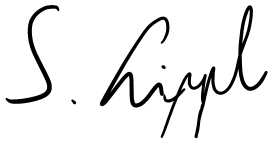
\includegraphics[scale=.5]{Bilder/Unterschrift.png}
\\\hline
Samuel Lippl, 7. Juni 2018
\end{tabular}

% -------------------------------------
% ABSTRACT
% -------------------------------------

\chapter*{Abstract}

\section*{Deutsch}
Neurale Netzwerke, zunächst als biologisches Modell des Gehirns eingeführt, haben sich als erfolgreiche Methode im Machine Learning etabliert, speziell wenn sie ihre Parameter mithilfe von Gradientenabstieg durch den Backpropagation-Algorithmus lernen. Dies hat die Frage aufgeworfen, ob unser Gehirn eine Art von Backpropagation implementiert. In dieser Bachelorarbeit stelle ich meinen Entwurf eines allgemeinen Modells neuraler Netzwerke vor und definiere in diesem Kontext den Backpropagation-Algorithmus und ein Modell neuronaler Komputation namens \textit{Predictive Coding}. Ich zeige, dass die mithilfe von \textit{Predictive Coding} angepassten Parameter unter gewissen Bedingungen gegen die Backpropagation-Parameter konvergieren und untersuche die biologische Plausibilität beider Methoden. Anschließend untersuche ich ein einfaches lineares \textit{Predictive Coding}-Modell genauer, das sich mit oder ohne \textit{a priori}-Verteilungen implementieren lässt. Ich zeige, dass \textit{Predictive Coding} mit immer höheren Varianzen der \textit{a priori}-Verteilungen gegen \textit{Predictive Coding} ohne \textit{a priori}-Verteilungen konvergiert.

\section*{English}
Although first introduced as a biological model of the brain, neural networks have found an important application as predictive algorithms in Machine Learning, most notably if they learn their parameters by gradient descent using the backpropagation algorithm. Its success has led to the discussion whether some form of backpropagation may be implemented in the brain. In this Bachelor's Thesis, I introduce a general framework of neural networks, in which I define the backpropagation algorithm and a model of neuronal computation that is called predictive coding. I prove conditions under which the parameters that are found by predictive coding converge to the ones that the backpropagation algorithm yields and discuss biological plausibility of both algorithms. I go on by studying a simple linear predictive coding model in more depth. This may be implemented with or without priors. I prove that predictive coding with priors that have increasingly high variance is equivalent to implementing predictive coding without priors.

% -------------------------------------
% TABLE OF CONTENTS
% -------------------------------------

\tableofcontents

% -------------------------------------
% INTRODUCTION
% -------------------------------------

\chapter{An Introduction to Computation in Machines, Brains and Mathematics}\label{ch:intro}
\pagenumbering{arabic}
\setcounter{page}{1}

\epigraph{What kind of computer is the brain?}{Sejnowski et al. \cite[][1300]{Sejnowski1988}}

In "Science and Statistics" \cite{Box1976}, George E. P. Box discusses the proper statistical methodology of tackling scientific problems. Although not at all concerned with this discipline, the paper gives a remarkably clear perspective on the field of computational neuroscience, not only with respect to its methodology but also with respect to its findings. The article therefore provides a proper compass, to position this Bachelor's Thesis at the intersection of statistics and Machine Learning, computational neuroscience and, evidently, mathematics.\\
Computational neuroscience is concerned with explaining "how electrical and chemical signals are used to represent and process information" \cite[][1299]{Sejnowski1988}. These problems are tackled by constructing theoretical models that are then checked by empirical data. Like the methodology of many fields of science, this strategy corresponds to the general principle of "iteration between theory and practice" \cite[][791]{Box1976} that Box discusses. It is important that this loop is closed: while omission of theory leads to the unjustified application of a few recipes to problems that are not suitable for these analyses -- a problem which Box calls "cookbookery" \cite[][797]{Box1976} --, "mathematistry", the "development of theory for theory's sake", has the tendency "to redefine the problem rather than solve it" \cite[][797]{Box1976}.\\
Besides ensuring a valid analysis of the data, theory plays a second important role in science: making certain that the obtained explanations actually contribute to our understanding. Sejnowski et al. \cite{Sejnowski1988} situate neural models on a spectrum from realistic to simplifying:
The Hodgkin-Huxley model of signal transmission \cite{Hodgkin1952} in nerves is a perfect example of a realistic model. At the level of a single neuron, it describes the formation of an action potential, an electrical signal that is used for long-distance information transmission. Realistic models, i. e. those that attempt to describe the physiological properties of a neuronal network, are insufficient for two reasons:\\
Firstly, a huge amount of data is needed to fit these models, especially at the network level, and the computational power to simulate entire networks at this level is immense. Secondly, even if the data were available -- which cannot be taken for granted, especially with concern to the human brain --, such a complex model may not enlighten our understanding of how the human brain works. A simplifying model may be better suited to illustrate important principles of information processing. These models are more concerned with how information is represented at a network level without considering the underlying physiological principles. Sejnowski et al. elaborate:
\begin{quote}
The study of simplifying models of the brain can provide a conceptual framework for isolating the basic computational problems and understanding the computational constraints that govern the design of the nervous system. \cite[][1300]{Sejnowski1988}
\end{quote}
This Bachelor's Thesis is concerned with the mathematical treatment of a popular simplifying model: neural networks. Keeping in mind the concerns that the previous arguments have raised, there are two balancing acts such a treatment has to accomplish:
\paragraph{Theory and Application}
Neural networks have originally been inspired by a biological model \cite{Rojas1996}. Inherent to the concept of a simplifying model is, however, the possibility that such a network may become "an end in itself" \cite[][1305]{Sejnowski1988}. This outcome may be framed as a mathematization in Box's terms. However, this development has been integrated into the field of Machine Learning that is concerned with the question "How may we recognize patterns?" instead of the neuroscientific question "How may our brain recognize patterns?". Neural networks have become a powerful tool in Machine Learning in a way that cannot be reframed as a model of our brain. In particular, the backpropagation algorithm has been a popular method to perform gradient descent in neural networks that is not likely to be implemented by our brain \cite{Liao2015}. Other Machine Learning algorithms are even less related to a biological model of learning.\\
Does this mean that such a development is unsuitable for further neuroscientific discussion? No. The differences between how Machine Learning algorithms may be implemented in the brain and how learning in the brain occurs in reality provides fruitful ground for new ideas in both disciplines and discussion whether differences are due to constraints of evolution or optimality.\\
One example for such a mechanism is the development of the \emph{predictive coding model} that was first proposed and successfully applied by Rao and Ballard \cite{Rao1999} to explain certain observations in the visual cortex. Friston developed and generalized this model (see, for instance, \cite{Friston2005}). Recently, Whittington and Bogacz presented predictive coding in its relation to the backpropagation algorithm \cite{Whittington2017}.\\
It is helpful for these discussions to have a general framework for neural networks, whether they are biologically plausible or not. I propose such a definition in chapter \ref{ch:theory}. It lays the groundwork for a mathematically rigorous and general introduction to backpropagation and predictive coding as well as their relations. This treatment may lead to predictive coding becoming just another end in itself. While empirical data is not of concern to a mathematical Bachelor's Thesis, I therefore introduce mathematical axioms in neural networks that have been supported by empirical data in order to prevent the mathematistry of my discussion of neural networks.
\paragraph{Generality and Conceptualization}
In the spirit of a mathematical analysis, chapter \ref{ch:theory} will introduce the concepts of prediction and learning in neural networks as well as backpropagation and predictive coding as generally as possible. This introduction shall be complemented by more restrictive conditions for which these networks will be simplified and easier to understand. An important goal of this Bachelor's Thesis is making definitions as general as possible  without losing their usefulness. Chapter \ref{ch:further-work} will conduct first more concrete analyses and consider possible directions of future investigations.\\
The principles I have set forth will guide my attempt to present neural networks such that the analysis provides the rigorosity and generality of a mathematical treatment, is sufficiently grounded in reality to contribute to computational neuroscience and sufficiently concrete to provide clear results (or perspectives of clear results).

% -------------------------------------
% GROUNDS OF THEORY
% -------------------------------------

\chapter{Feedforward Neural Networks and Predictive Coding}\label{ch:theory}

This chapter will be concerned with introducing general neural networks. Section \ref{sec:theory-structure} will cover their structure. We will go on to states of neural networks in \ref{sec:theory-states} before introducing learning in neural networks in \ref{sec:theory-learning}. The specific theory of learning by backpropagation and predictive coding will be introduced alongside the more general groundwork.

\section{Structure of Neural Networks}\label{sec:theory-structure}

\begin{Par}[Neural Networks as Graphs]\label{theory-structure:intro}
Neural networks may be based on graphs where we refer to the nodes as \emph{Processing Units} (PU) and to the edges as \emph{Unit Connections} (UC). We can therefore use an adjacency matrix that specifies for each pair of PUs whether there is a connection between them (see \thref{par:adjacency}) to specify the neural network.\\
Moreover, there is a set of parameters that specify the behaviour of a neural network. As most of these parameters are directly connected to a UC, we will define a neural network by its \emph{weight matrix} which is a weighted adjacency matrix. However, we now face a difficulty concerning the relationship between the structure and the parameters. Generally, a connection between two PUs is indicated by a non-zero entry in the adjacency matrix while an entry of zero indicates that the two PUs are not connected. However, what if a connection between two PUs is weighted by zero? The difference between this case and no connection at all will become important in section \ref{sec:theory-learning}: a connection with weight zero may change during learning whereas two unconnected PUs will always remain unconnected. Moreover, how may we define a neural network where we know the UCs but have no specification of their weights?\\
Subsection \ref{subsec:theory-structure-matrix} presents a solution to these difficulties. Subsection \ref{subsec:theory-structure-forms} provides some vocabulary to talk about neural networks by introducing the standardized layerization. Subsequently, subsection \ref{subsec:theory-structure-predicode} will first introduce concepts from predictive coding, namely the generative model. This section will conclude with \ref{subsec:theory-structure-other} where we will embed the provided definition in the context of literature and will discuss the concept of \emph{parallelity} and its connection to neural networks.
\end{Par}

\subsection{The Network Matrix}\label{subsec:theory-structure-matrix}

\begin{Def}[$\const$-$\var$-extension of a set]
If $A$ is a set, we define its \emph{$\const$-$\var$-extension} 
\begin{equation}\label{eq:c-v-extension}
A_{\const,\var}:=\left(A\times\left\{\const,\var\right\}\right)\cup\{\var_A\},
\end{equation}
where we denote for any $a\in A$
\begin{equation}\label{eq:not-c-v}
a_{\const}\equiv(a,\const)\quad a_{\var}\equiv(a,\var),
\end{equation}
and may omit the subscripts when they become clear from context.\\
We will treat $0_{\const}$ like an ordinary zero, i. e. a number in a matrix is omitted if and only if it is $0_{\const}$ and a diagonal matrix only has $0_{\const}$ entries that are not on its diagonal.\\
If $a\in A\times\{\const\}$, then $a$ is \emph{constant} and we write $\St(a)=\const$ ($\St$ is an abbreviation of \emph{status}). If $a\in\left(A\times\{\var\}\right)\cup\{\var\}$, then $a$ is \emph{variable} and we write $\St(a)=\var$. Finally, we denote the value of $a$ by $\Val(a_{\const})=\Val(a_{\var})=a$ where $\Val(\var)$ is not defined.
\end{Def}

\begin{Def}[$\const$-$\var$-extension of a function]
Consider sets $I, A^i$, where $i\in I$, $B$ and $C$.
\begin{enumerate}[a)]
\item
We define the \emph{passive} $\const$-$\var$-extension of a function $f:\prod_{i\in I}A^i\to B$ by
\begin{equation}\label{eq:domain-extension}
\begin{aligned}
f:\prod_{i\in I}A^i_{\const,\var}&\to B_{\const,\var},\\
\Val\left(f(a)\right)&:=\begin{cases}
f\left(\left(\Val(a_i)\right)_{i\in I}\right)&\text{ if }\neg\underset{i\in I}{\exists}a_i=\var,\\
c&\text{ if }\left(\underset{i\in I}{\exists}a_i=\var\right)\wedge f\left(\left(\Val(a_i)\right)_{i\in I:a_i\ne\var},\cdot\right)\equiv c,\\
\var&\text{ else},
\end{cases}\\
\St\left(f(a)\right)&:=\begin{cases}
\const&\text{ if }\underset{i\in I}{\forall}\St(a_i)=\const,\\
\var&\text{ else }.
\end{cases}
\end{aligned}
\end{equation}
We will denote the passive extension by the same symbol as the original function.
\item
We define the \emph{active} $\const$-$\var$-extension of a function
\[
f:\prod_{i\in I}A^i\times C\to \prod_{i\in I}A^i\times B, 
\begin{pmatrix}
a\\c
\end{pmatrix}
\mapsto
\begin{pmatrix}
\left(f_i(a,c)\right)_{i\in I}\\
f_B(a,c)
\end{pmatrix}
\qquad
\]
in $A:=(A_i)_{i\in I}$ by
\begin{equation}
\begin{aligned}
f_{\const,\var:A}:\prod_{i\in I}A^i_{\const,\var}\times C&\to \prod_{i\in I}A^i_{\const,\var}\times B,\\
f_{\const,\var:A}(a,c)_i&:=
\begin{cases}
f(a,c)_i & \St(a_i)=\var,\\
a_i & \St(a_i)=\const.
\end{cases}
\end{aligned}
\end{equation}
If $C=\emptyset$, we simply write $f_{\const,\var}$.
\end{enumerate}
\end{Def}

\begin{Par}[Passive Extension]
The passive extension allows application of a function $f$ to $\const$-$\var$-extended values. $f(a)$ is constant if and only if every argument is constant. Generally, the value of the extended $f$ is simply the value of the original $f$ when applied to the values of the arguments, for instance:
\[
1_{\const}+2_{\var}=(1+2)_{\var}=3_{\var}.
\]
This is covered by the first case of the definition. Things only get messy when the value of an argument is unknown. In this case, generally, $f(a)$ is unknown as well, for instance:
\[
1_{\const}+\chi=\chi.
\]
The only exception is given by a function that is constant in the unknown argument, for instance:
\[
0_{\const}\cdot\chi =0_{\var}.
\]
\end{Par}

\begin{Par}[Active Extension]
The active extension ensures that no constant value will be changed. This will, for instance, be useful in the learning function, where we do not want $0_{\const}$ to change as this value encodes that there is no connection between two PUs, as we discussed in \thref{theory-structure:intro}.
\end{Par}

\begin{Par}[Adjacency Matrix]\label{par:adjacency}
An adjacency matrix has the following connection to a graph: Given a graph $\mathcal{G}:=(\mathcal{V},\mathcal{E}),\mathcal{E}\subseteq\mathcal{V}\times\mathcal{V}$, we may write $\mathcal{G}$ as a matrix $W\in\{0,1\}^{\mathcal{V}\times\mathcal{V}}$ where $W_{v,w}=1\Leftrightarrow (v,w)\in\mathcal{E}$.\\
If we consider weighted edges, we may generalize the notion to a matrix $W\in A^{\mathcal{V}\times\mathcal{V}}$ on a ring $A$ where $W_{v,w}\ne 0$ specifies the weight of edge $(v,w)\in\mathcal{E}$ and an edge with weight zero is synonymous with no edge at all. It is therefore important that the use of these weights is defined in an appropriate way.\\
We can further extend the notion of an adjacency matrix to $W\in A^{\mathcal{V}\times\mathcal{V}}_{\const,\var}$ where
\begin{equation}\label{eq:matrix-graph}
(v,w)\in\mathcal{E}\Leftrightarrow W_{v,w}\ne 0_{\const}.
\end{equation}
\end{Par}

\begin{Def}[Graph Relations]
If $\mathcal{G}:=(\mathcal{V},\mathcal{E})$ is a graph and $v,w\in\mathcal{V}$, we introduce the following three relations:
\begin{align}
v\to_{\mathcal{E}} w&\equiv (v,w)\in\mathcal{E},\\
v\leftarrow_{\mathcal{E}} w &\equiv w\to_{\mathcal{E}} v,\\
v\conn_{\mathcal{E}} w &\equiv v\to_{\mathcal{E}} w\vee v\leftarrow_{\mathcal{E}} w,
\end{align}
where we will often leave the subscript implicit.\\
We define their transitive closures $\to^*,\leftarrow^*,\conn^*$. If $v\to^* w$ (resp. $v\to w$) we say that $v$ precedes (resp. directly precedes) $w$ and $w$ succeeds (resp. directly succeeds) $v$. $v$ and $w$ are connected (resp. directly connected) if and only if $v\conn^* w$ (resp. $v\conn w$).\\
We will denote the set of directly preceding nodes by $\to v$ and the set of directly succeeding nodes by $v\to$.
\end{Def}

\begin{Def}[Connected Graph]
A graph is called \emph{connected} if and only if all its nodes are connected.
\end{Def}

\begin{Def}[Neural Network I: Topological Structure]
Consider a ring $A$ and a finite set $\mathcal{V}\ne\emptyset$. A tupel $\mathfrak{N}=(\mathcal{V},\theta), \theta\in A_{\const,\var}^{\mathcal{V}\times\mathcal{V}}$ is called a neural network if and only if the graph corresponding to $\theta$ is connected.
\end{Def}

\begin{Rem}
The condition that neural networks have to be connected is not a restriction because if there are two unconnected parts in the network, we can simply consider these parts as separate networks.
\end{Rem}

\begin{Not}[Adjacency Matrix]
While generally using the common matrix notations, we will refer to the elements of $\theta$ in a slightly different way. The entry in row $v$ and column $w$ is denoted by $\theta_{v\to w}$, the entries in row $v$ are denoted by $\theta_{v\to}$ and the entries in column $w$ are denoted by $\theta_{\to w}$. For $V,W\subseteq\mathcal{V}$
\[
\theta_{V\to W}\equiv\left(\theta_{v\to w}\right)_{v\in V,w\in W}\in\mathbb{R}^{V\times W}.
\]
Finally, we define the identity matrix $I$ on an arbitrary domain, i. e. for sets $M, N$, we define
\[
I_{M\to N}:=(\delta_{mn})_{m\in M,n\in N},
\]
where $\delta_{ij}$ is the Kronecker delta.
\end{Not}

\begin{Not}
For any family $(a_i)_{i\in I}$, if $J\subseteq I$, we denote $a_J\equiv(a_j)_{j\in J}$. If there is a set of functions $f_i:A_i\to B_i$, $i\in I$, and $a\equiv(a_i)_{i\in I},a_i\in A_i$, we denote $f(a)\equiv\left(f_i(a_i)\right)_{i\in I}$.
\end{Not}

\begin{Def}[States]
Given a neural network $\mathfrak{N}=(\mathcal{V},\theta)$, we will call
\[
s\in S[\mathfrak{N}]:=A^{\{i,o\}\times\mathcal{V}}
\]
a \emph{state} of $\mathfrak{N}$. If $(k,v)\in\{i,o\}\times\mathcal{V}$, we denote the $(k,v)$-entry in $s$ by $s^{v:k}$. We refer to $s^{v:i}$ as the \emph{input value} of $v$ and $s^{v:o}$ as the \emph{output value} of $v$.\\
Furthermore, we denote, for $v\in\mathcal{V},V\subseteq\mathcal{V}$ and $k\in\{i,o\}$
\[
s^{V:k}\equiv\left(s^{v:k}\right)_{v\in V},
\quad
s^{:k}\equiv s^{\mathcal{V}:k},
\quad
s^{v:}\equiv\left(s^{v:i},s^{v:o}\right),
\quad
s^{V:}\equiv\left(s^{v:}\right)_{v\in V}.
\]
We define the \emph{$\const$-$\var$-extended state} $s\in S_{\const,\var}[\mathfrak{N}]:=A_{\const,\var}^{\{i,o\}\times\mathcal{V}}$.\\
Using the analogous notation, we define the \emph{state} of $\mathfrak{N}$ in $V\subseteq\mathcal{V}$ by 
\[
S^V[\mathfrak{N}]:=A^{\{i,o\}\times V},
\quad
S^{V:k}[\mathfrak{N}]:=A^{\{k\}\times V},
\]
and the \emph{$\const$-$\var$-extended state} by
\[
S^V_{\const,\var}[\mathfrak{N}]:=A^{\{i,o\}\times V}_{\const,\var},
\quad
S^{V:k}_{\const,\var}[\mathfrak{N}]:=A^{\{k\}\times V}_{\const,\var}.
\]
\end{Def}

\begin{Def}[Neural Network II: Functional Structure]
Let $\mathfrak{N}=(\mathcal{V},\theta)$ be a neural network.
Consider a set of \emph{global parameters} $\Lambda$, \emph{unit functions} $f\equiv\left(f^u\right)_{u\in\mathcal{V}}$ and \emph{integrative functions} $g\equiv\left(g^u\right)_{u\in\mathcal{V}}$.
The tupel $(\Lambda,f,g)$ is called the \emph{functional structure} of $\mathfrak{N}$ if and only if, for all $u\in\mathcal{V}$,
\begin{equation}
f^u:A\to A,\quad s^u\mapsto f^u(s^u),
\end{equation}
and every $g^u$ is defined as the active extension of some $\tilde{g}^u$ in $S^{\{u\}:i}[\mathfrak{N}]$ such that
\begin{equation}
\tilde{g}^u:S[\mathfrak{N}]\times A_{\const,\var}^{\mathcal{V}\times\mathcal{V}}\times\Lambda_{\const,\var}\to A,
\quad
(s^{:o},\theta,\lambda)\mapsto \tilde{g}^u_{\theta,\lambda}(s^{:o}),
\end{equation}
only depends on $\left\{s^v:\Val(\theta_{v\to u})=0\right\}$, $\theta_{\to u}$ and $\lambda$.\\
By convention, we define $g$ by $\tilde{g}$ and leave its extension implicit.
\end{Def}

\begin{Rem}
We cannot simply demand that $\tilde{g^u}$ only depend on the state $s^{\to u}$ as we do not want it to depend on values where $\theta_{v\to u}=0_{\var}$.
\end{Rem}

\begin{Par}[Integrative Functions]
A unit's integrative function summarizes the output of a unit's directly preceding nodes. The first argument therefore provides the values of these nodes, the second argument provides the weight matrix $\theta$ and the third argument is a set of global parameters. How neural networks may adopt concrete states will be of concern in section \ref{sec:theory-states}.
\end{Par}

\begin{Par}[Unit Functions]
The unit functions relate the summarized input to a node $s^{u:i}:=g^u_{\theta,\lambda}(s)$ to its output value $s^{u:o}:=f^u(s^{u:i})$.
\end{Par}

\begin{Def}[Additive Neural Networks]
A neural network $\mathfrak{N}=(\mathcal{V},\theta)$ is called \emph{straight} if and only if
\[
\underset{v,w\in\mathcal{V}}{\forall}v\to w\Rightarrow\neg\underset{u\in\mathcal{V}}{\exists}v\to u\to^*w.
\]
A straight neural network $\mathfrak{N}=(\mathcal{V},\theta)$ with functional structure $(\Lambda,f,g)\equiv(f,g),\Lambda=\emptyset$ is called \emph{additive} if and only if
\begin{equation}
g_{\theta}(s^{:o})=\theta^Ts^{:o}.
\end{equation}
$\mathfrak{N}$ is called \emph{general additive} neural network if and only if, for all $u\in\mathcal{V}$, there are sets $i_u,o_u\subseteq \mathcal{V}\setminus i_u$ such that
\begin{equation}
g^u_{\theta}(s^{i_u:o},s^{o_u:o})=\theta_{i_u\to u}^Ts^{i_u:i}+\theta_{o_u\to u}^Ts^{o_u:o}.
\end{equation}
\end{Def}

\begin{Par}
Straightness of neural networks ensures that there are no hidden dependencies. If $v$ is not only directly connected to $w$ but also indirectly, $g^w$ does not specify the entire dependence on the value of $v$. It is therefore crucial for an additive network to be straight; if not, the influence of the preceding nodes would seem additive according to $g$ but hidden dependencies may render it non-linear.
\end{Par}

\subsection{Layerization}\label{subsec:theory-structure-forms}

\begin{Par}[Layers of Neural Networks]
Many neural networks are defined in layers where $\mathcal{V}:=V^{(0)}\dot{\cup}\dotsb\dot{\cup}V^{(L)}$ and $v\to w\Leftrightarrow \underset{l\le L}{\exists}\left(v\in V^{(l)}\wedge w\in V^{(l+1)}\right)$. These layers can be extended to a class of neural networks called \emph{feedforward neural networks}. This subsection is concerned with finding and characterizing these layers, a process called \emph{layerization}.
\end{Par}

\begin{Not}
To simplify the notation of layers we define, for $l,l_1,\dotsc,l_n\in\{0,\dotsc,L\}$,
\[
V^{(\square l)}:=\bigcup_{k\in\{0,\dotsc,L\}:k\square l}V^{(k)},
\]
where $\square$ is some relation, e. g. $\le$, and
\[
V^{(l_1,\dotsc,l_n)}:=\bigcup_{i=1}^nV^{(l_i)}.
\]
\end{Not}

\begin{Def}[Feedforward Neural Networks]
A neural network is called feedforward if and only if its graph is acyclical. Feedforwardness is therefore a topological property.
\end{Def}

\begin{Pro}[Characterization of feedforward neural networks]\label{pro:chara-feedforward}
Let $\mathfrak{N}=(\mathcal{V},\theta)$ be a neural network. Then, the following conditions are equivalent:
\begin{enumerate}[(i)]
\item
$\mathfrak{N}$ is feedforward,
\item
$\to$ is acyclical,
\item
There are layers $V^{(0)},\dotsc,V^{(L)}$ such that $\mathcal{V}=V^{(0)}\dot{\cup}\dotsb\dot{\cup}V^{(L)}$ and 
\begin{equation}
V^{(l)}\ni v\to w\in V^{(k)}\Rightarrow l<k,
\end{equation}
\item
There is a function $\pi:\mathcal{V}\to\left\{1,\dotsc,|\mathcal{V}|\right\}$ such that
\begin{equation}\label{eq:chara-feedforward-iv}
v\to w\Rightarrow \pi(v)<\pi(w),
\end{equation}
\item
There is a function $\pi:\mathcal{V}\to\left\{1,\dotsc,|\mathcal{V}|\right\}$ such that
\begin{equation}\label{eq:chara-feedforward-v}
\theta_{\pi}:=\left(\theta_{v\to w}\right)_{\pi(v),\pi(w)}
\end{equation}
is an upper triagonal matrix.
\end{enumerate}
\end{Pro}

\begin{Bew}
\textit{(i)$\Leftrightarrow$(ii)}
Follows by definition.\\
\textit{(i)$\Rightarrow$(iii)}
is a special case of \thref{cor:standardized-layerization-feedforward}\footnote{
Note that we do not use the proposition in any proof until then.}.\\
\textit{(iii)$\Rightarrow$(iv)}
Assign numbers in $\{1,\dotsc,|\mathcal{V}^{(0)}|\}$ to the elements of $\mathcal{V}^{(0)}$. For any $0<l\le L$ assign numbers in $\left\{\sum_{j=1}^{l-1}|\mathcal{V}^{(j)}|+1,\dotsc,\sum_{j=1}^{l}|\mathcal{V}^{(j)}|\right\}$ to the elements of $\mathcal{V}^{(l)}$. Then $v\to w$ where $v\in\mathcal{V}^{(l)}$ and $w\in\mathcal{V}^{(k)}$ implies $l<k$ and therefore 
\[
\pi(v)\le \sum_{j=1}^{l}|\mathcal{V}^{(j)}|<\sum_{j=1}^{l}|\mathcal{V}^{(j)}|+1\le \sum_{j=1}^{k}|\mathcal{V}^{(j)}|+1\le\pi(w).
\]
\textit{(iv)$\Rightarrow$(v)}
We simply prove that (\ref{eq:chara-feedforward-iv}) implies (\ref{eq:chara-feedforward-v}). This becomes clear from the fact that 
\[
(\theta_{\pi})_{\pi(v),\pi(w)}\ne0_{\const}\Rightarrow\theta_{v\to w}\ne0_{\const}\Rightarrow v\to w\Rightarrow\pi(v)<\pi(w),
\]
which is the definition of an upper triagonal matrix.\\
\textit{(v)$\Rightarrow$(iv)}
We now prove that (\ref{eq:chara-feedforward-v}) implies (\ref{eq:chara-feedforward-iv}). This follows from
\[
v\to w\Rightarrow(\theta_{\pi})_{\pi(v),\pi(w)}\ne0_{\const}\Rightarrow\pi(v)<\pi(w).
\]
\textit{(iv)$\Rightarrow$(ii)}
Clearly, (\ref{eq:chara-feedforward-iv}) could not hold if $\to$ contained a cycle.
\end{Bew}

\begin{Par}
Condition (iii) has a more universal appeal which we will discover now. These layers can be specified either by a partition of $\mathcal{V}$ or a transitive total order $\preceq$. After proving their equivalence, we go on to provide the definition of different kinds of layerizations.
\end{Par}

\begin{Def}[Layerization]\label{def:layerization}
A transitive total (but not necessarily antisymmetric) order $\preceq$ on $\mathcal{V}$ is called layerization. We denote
\[
v\prec w\equiv v\preceq w\wedge w\npreceq v, \quad v\simeq w\equiv v\preceq w\wedge w\preceq v.
\]
A connection $v\to w$ is called
\begin{itemize}
\item
\emph{forward} if and only if $v\prec w$,
\item
\emph{lateral} if and only if $v\simeq w$,
\item
\emph{backward} if and only if $v\succ w$.
\end{itemize}
The corresponding equivalence classes $\mathcal{V}/{\simeq}$ are called \emph{layers}. As $\preceq$ is transitive, we may define $\preceq$ on $\mathcal{V}/{\simeq}$ by
\begin{equation}
V\preceq W\equiv\underset{v\in V, w\in W}{\forall}v\preceq w\equiv\underset{v\in V,w\in W}{\exists}v\preceq w.
\end{equation}
As $\preceq$ is antisymmetrical on $\mathcal{V}/{\simeq}$, we can now notate the layerization as a partition $\mathcal{V}=\dot{\bigcup}_{l=0}^LV^{(l)}$ where
\[
\mathcal{V}/{\simeq}=\left\{V^{(l)}:0\le l\le L\right\},
\quad 
V^{(l)}\prec V^{(l+1)},
\]
which yields the layerization form of \thref{pro:chara-feedforward}.\\
We will call $\preceq$ the \emph{ordinal} and the partition $\left(V^{(l)}\right)_{0\le l\le L}$ the \emph{set notation} of the layerization. $L$ is called the \emph{depth} of the layerization.
\end{Def}

\begin{Pro}\label{pro:layerization-11}
There is a one-to-one correspondence between ordinal and set layerization.
\end{Pro}

\begin{Bew}
The function from ordinal to set layerization has already been given by \thref{def:layerization}. On the other hand, if there is a set layerization, the order that is defined by
\[
V^{(l)}\ni v\preceq w\in V^{(k)}\Leftrightarrow l\le k,
\]
is total and transitive.\\
We now only have to prove that the ordinal notation converted to the set notation converted to the ordinal notation provides indeed the same layerization. Let $v,w\in\mathcal{V}$. WLOG, suppose that $v\preceq w$. Then $v\prec w\xor v\simeq w$ where $\xor$ is the exclusive disjunction. If $v\prec w$, there are different equivalence classes $V\ne W$ such that $v\in V,w\in W$. As $v\prec w$, $V\prec W$ and therefore layer $V$ comes before layer $W$. This, again, yields $v\prec w$. The other case, $v\simeq w$, works in an analogous way.
\end{Bew}

\begin{Par}
By \thref{pro:layerization-11}, we will use the relational and set form of layerization interchangeably from now on. The next definition provides an important stepping stone towards the function of layerizations by formalizing the notion of forward, lateral and backward connections by a relation: the flow\footnote{
which is different from the standard flow in graph theory as defined, for instance, in \cite[][149]{Diestel2017}}. The main motivation behind this is \thref{def:layerization-equivalence}.
\end{Par}

\begin{Def}
Given a layerization $\preceq$ of a network $\mathfrak{N}$, we define the following relations which we will refer to as the \emph{flow} of $\mathfrak{N}$.
\begin{equation}
\begin{aligned}
v\trianglerighteq w&\equiv 
v\conn w\wedge v\preceq w,&
v\trianglelefteq w&\equiv w\trianglerighteq v,&
v\smallsquare w&\equiv v\trianglerighteq w\wedge v\trianglelefteq w,\\
v\triangleright w &\equiv v\trianglerighteq w\wedge\neg(v\smallsquare w),&&&
v\triangleleft w&\equiv w\triangleright v.
\end{aligned}
\end{equation}
\end{Def}

\begin{Lem}
$\underset{v,w\in\mathcal{V}}{\forall}v\conn w\Leftrightarrow v\smallsquare w\xor v\triangleright w\xor v\triangleleft w$ where $\xor$ is an exclusive disjunction.
\end{Lem}

\begin{Bew}
Suppose $\neg(v\conn w)$. It is evident from its definition that there is no flow between $v$ and $w$ in this case. In turn, if $v\conn w$, the totality of $\preceq$ implies the trichotomy and the definition of the strict inequalities implies that the trichotomy is exclusive.
\end{Bew}

\begin{Def}
A layerization $\preceq$ on $\mathcal{V}$ is called
\begin{enumerate}[a)]
\item
\emph{minimal} if and only if there is a sequence $v_0,\dotsc,v_L$ such that $v_l\in\mathcal{V}^{(l)}$ for all $l=0,\dotsc, L$ and $v_l\triangleright v_{l+1}$ for all $l=0,\dotsc, L-1$,
\item
\emph{spanned} if and only if the minimal and maximal values of $\preceq$ and $\triangleright^*$, the transitive closure of $\triangleright$, are identical, 
\item
\emph{leftwards} (resp. \emph{rightwards}) \emph{anchored} if and only if for any $v_l\in\mathcal{V}^{(l)}$ there is a sequence $v_0,\dotsc,v_{l-1}$ such that for all $k=0,\dotsc, l-1$, $v_k\triangleright v_{k+1}$ and $v_k\in V^{(k)}$ (resp. a sequence $v_{l+1},\dotsc, v_L$ such that for all $k=l,\dotsc, L-1$, $v_k\triangleright v_{k+1}$ and $v_{k+1}\in V^{(k+1)}$).
\end{enumerate}
\end{Def}

\begin{Lem}
An anchored layerization is minimal.
\end{Lem}

\begin{Bew}
If the layerization is leftwards anchored, set $l=L$. If the layerization is rightwards anchored, set $l=0$.
\end{Bew}

\begin{Def}\label{def:layerization-equivalence}
Two layerizations $\preceq_1$, $\preceq_2$ of a neural network $\mathfrak{N}$ are called \emph{equivalent} (Not.: $\preceq_1\sim\preceq_2$) if and only if the flow remains identical.
\end{Def}

\begin{Par}
Layerizations provide different perspectives on a neural network. Generally, however, we want our notion of forward, lateral or backward connections (especially whether a given network is feedforward) to remain invariant. Equivalent layerizations ensure such invariance.
\end{Par}

\begin{Lem}\label{lem:depth}
Given a layerization $\preceq$ and a chain $v_0\triangleright\dotsb \triangleright v_n$ where $v_0\in V^{(l)}$ and $v_n\in V^{(k)}$, we obtain $n\le k-l$.
\end{Lem}

\begin{Bew}
Proof by induction on $k-l$. By definition, $v_n$ has to lie in a higher layer than $v_0$ if $v_0\ne v_n$. Therefore, if $k<l$, such a chain is not possible and if $k=l$, $n=0$.\\
If $k-l\ge 1$, consider $v_{n-1}\in V^{(k')}$ and observe that $k'<k$ and therefore $k'\le k-1$. Then, by induction hypothesis, $n-1\le k'-l\le k-1-l$ and therefore $n\le k-l$. 
\end{Bew}

\begin{The}[Standardized Layerization]\label{the:standardized-layerization}
For every flow $\triangleright$ of a neural network $\mathfrak{N}$, there is a unique minimal spanned and leftwards (resp. rightwards) anchored layerization $\preceq_l$ (resp. $\preceq_r$) such that the flow of $\preceq_l$ (resp. $\preceq_r$) is $\triangleright$. We call $\preceq_l$ (resp. $\preceq_r$) \emph{leftwards} (resp. \emph{rightwards}) \emph{standardized layerization}.
\end{The}

\begin{Bew}
If there are no $v,w\in\mathcal{V}$ such that $v\triangleright w$, a minimal layerization must necessarily have depth $L=0$ and we therefore obtain $V^{(0)}=\mathcal{V}$ and uniqueness for both the leftwards and the rightwards standardized layerization. This is equivalent to the original layerization: if $v\smallsquare w$, then $v\conn w$ and therefore $v\smallsquare_lw$ and $v\smallsquare_rw$. This proves equivalence as there are no $v,w$ such that $v\triangleright w$. The minimal and maximal values of $\preceq_l$, $\preceq_r$ and $\triangleright^*$ are given by $V^{(0)}=V^{(L)}=\mathcal{V}$ and therefore, $\preceq_l$ and $\preceq_r$ are spanned. Anchoredness is rendered trivial which proves the first case. We will therefore choose $v,w\in\mathcal{V}$ such that
\begin{equation}\label{eq:standardized-layerization-1}
v\triangleright w
\end{equation}
and define $V^{(0)}$ as the minimal values of $\triangleright^*$ and $V^{(\max)}$ as the maximal values of $\triangleright^*$. These sets are uniquely defined as this is equivalent to the condition that the layerization is spanned. The two sets are also disjoint. In order to prove that, we prepare the following lemma:

\begin{BLem}\label{standardized-layerization-2}
If $u\in V^{(0)}\cap V^{(L)}$,
\[
\underset{v\in\mathcal{V}}{\forall}u\smallsquare^* v.
\]
\end{BLem}

\begin{BBew}
Let $v\in\mathcal{V}$. By definition of neural networks, $u\conn^*v$. As $\mathcal{V}$ is finite, the definition of the transitive closure directly implies that there is some chain $v_1,\dotsc,v_{n-1}\in\mathcal{V}$ such that
\[
u\conn v_1\conn\dotsb\conn v_{n-1}\conn v.
\]
We prove $u\smallsquare^*v$ by induction on $n$.
If $n=1$, $u\conn v$ and therefore $u\triangleright v\vee u\smallsquare v\vee u\triangleleft v$. As $u$ is both a maximal and a minimal element, this implies $u\smallsquare v$ and therefore $u\smallsquare^* v$.\\
Now suppose $n>1$. By induction hypothesis, we know that $u\smallsquare^* v_{n-1}$. On the other hand, as $v_{n-1}\conn v$. As $\trianglerighteq^*$ is transitive, $v_{n-1}$ is therefore also maximal. By the same argument as above, $v_{n-1}\smallsquare^* v$ and therefore $u\smallsquare^* v$.
\end{BBew}

Now, suppose there is some $u\in V^{(0)}\cap V^{(L)}$. Using the PUs $v,w$ from (\ref{eq:standardized-layerization-1}), we conclude by \thref{standardized-layerization-2} $v\smallsquare^* u\smallsquare^* w$ and therefore $v\smallsquare^* w$ which is a contradiction to (\ref{eq:standardized-layerization-1}) and proves that $V^{(0)}\cap V^{(L)}=\emptyset$.\\
We apply the following algorithm to obtain the remaining layers if we want a leftwards anchored layerization:
\begin{enumerate}
\item
Set $t=0$ and $R^{(0)}:=\mathcal{V}\setminus\left(V^{(0)}\cup V^{(L)}\right)$,
\item
While $R^{(t)}\ne\emptyset$:
\begin{enumerate}
\item
Define $V^{(t+1)}$ as the set of minimal values in $R^{(t)}$,
\item
Set $R^{(t+1)}:=\mathcal{R}^{(t)}\setminus V^{(t+1)}$,
\item
Increment $t$ by $1$,
\end{enumerate}
\item
Set $L:= t$.
\end{enumerate}
Clearly, this yields a partition. As $R^{(L)}$ is empty, every $v\in\mathcal{V}$ is in some layer and the construction ensures that the sets $V^{(0)},\dotsc,V^{(L-1)}$ as well as the sets $V^{(1)},\dotsc,V^{(L)}$ are pairwise disjoint where we have already proven that $V^{(0)}\cap V^{(L)}=\emptyset$.\\
The layerization is leftwards anchored as we prove by induction on $l$ in the definition: For $v_0\in V^{(0)}$, the criterion is trivial. If $l=1$, we obtain some $v_1\in V^{(1)}$. As $v_1\notin V^{(0)}$, it is not minimal and there is some $v_0\in\mathcal{V}$ such that
\[
v_0\triangleright v_1.
\]
As $v_1$ is minimal in $R^{(0)}=\mathcal{V}\setminus\left(V^{(0)}\cup V^{(L)}\right)$ we conclude $v_0\in V^{(0)}\cup V^{(L)}$. As $v_0$ is not maximal, $v_0\in V^{(0)}$ and we have found our chain.
Finally, if $l>1$ and $v_l\in V^{(l)}$, we know that $v_l$ was minimal in $R^{(l-1)}$ but not in $R^{(l-2)}$. Therefore, there must be some $v_{l-1}\in V^{(l-1)}$ such that $v_{l-1}\triangleright v_l$ and the existence of the chain follows by induction hypothesis.\\
On the other hand, the layers $V^{(1)},\dotsc,V^{(L-1)}$ are uniquely defined by the condition that the layerization must be leftwards anchored. Take any $v\in V^{(l)}$, $1\le l\le L-1$, and suppose that there is an equivalent, leftwards anchored and spanned layerization $\preceq'$ with set notation $V'^{(0)},\dotsc,V'^{(L')}$ such that $v\in V'^{(k)},k\ne l$. If $k<l$, $\preceq'$ would be impossible by \thref{lem:depth} because there is a chain $V'^{(0)}=V^{(0)}\ni v_0\triangleright\dotsb\triangleright v_{l-1}\triangleright v\in V'^{(k)}$ as $\preceq_l$ is leftwards spanned. If $k>l$, the existence of $\preceq'$ would imply, by the same argument, that $\preceq_l$ is impossible. As we have already shown that $\preceq_l$ is well-defined, this is a contradiction. Therefore, $k=l$ and $\preceq_l$ is uniquely defined.\\
An analogous method shows that $\preceq_r$ is unique and well-defined where we use a top-down instead of a bottom-up approach with the algorithm and all arguments thereafter.
\end{Bew}

\begin{Cor}
For every layerization $\preceq$ on a neural network $\mathfrak{N}$, there is a unique equivalent leftwards or rightwards standardized layerization.
\end{Cor}

\begin{Bew}
The layerization is provided by the flow defined by $\preceq$ and \thref{the:standardized-layerization}.
\end{Bew}

\begin{Cor}\label{cor:standardized-layerization-feedforward}
If $\mathfrak{N}$ is a feedforward network and $v\trianglerighteq w\equiv v\to w$, there is a unique leftwards or rightwards standardized layerization. Canonically, we consider one of these layerizations and only specify which one, if it makes a difference.
\end{Cor}

\begin{Pro}[Depth of Layerizations]
Let $\mathfrak{N}$ be a neural network. Given a layerization $\preceq$ of $\mathfrak{N}$, if $\preceq'$ and $\preceq''$ are equivalent minimal layerizations with depths $L'$ and $L''$, we obtain 
\[
L'=L''.
\]
We call $L'$ the depth of $\mathfrak{N}$. Furthermore, any equivalent layerization that is not minimal has a depth of at least $L'+1$.
\end{Pro}

\begin{Bew}
It is sufficient to prove $L'\le L''$. As $\preceq'$ is minimal, we can find $v_0,\dotsc,v_{L'}$ such that $V'^{(0)}\ni v_0\triangleright\dotsb\triangleright v_{L'}\in V'^{(L')}$. Considering $\preceq''$, let $v_0\in {V''}^{(k)}$ and $v_{L'}\in {V''}^{(l)}$. By the invariance of the flow under equivalent layerizations and \thref{lem:depth}, $L'\le l-k\le L''$. This also proves that any equivalent layerization (whether it is minimal or not) has a depth of at least $L'$. If we have proven that any layerization of depth $L'$ is minimal, the second part of the proposition is proven. Consider, again, the chain $v_0,\dotsc, v_{L'}$. Let $v_0\in V^{(k)}$ according to the equivalent layerization. If $k>0$, it is easy to see that the remaining chain yields a contradiction. Therefore, $v_0\in V^{(0)}$. Analogously, we can prove by induction that $v_l\in V^{(l)}$ and the layerization is therefore minimal.
\end{Bew}

\begin{Par}
We have therefore found a way to layerize any feedforward network in a sensible way. On the other hand, when we extend the feedforward network to a more general network, we can still talk about the network's layers in a standardized manner. The next section lays the groundwork for this very necessity.
\end{Par}

\subsection{The Generative Model}\label{subsec:theory-structure-predicode}

\begin{Def}[Stochastic Networks]
Consider a probability space $(\Omega,\mathcal{F},\mathbb{P})$. We define a \emph{stochastic network} $\mathfrak{S}:=(\mathcal{V},\theta)$ with functional structure $(\Lambda,f,g)$, $\Lambda=\Omega\times\Lambda'$ such that, for all $u\in\mathcal{V}$,
\begin{equation}
g^u_{\theta,(\omega,\lambda')}\left(s\right)=g^u_{\theta,\lambda'}(\omega),
\end{equation}
where
\[
g^u_{\theta,\lambda'}:\Omega\to\mathbb{R}
\]
is a random variable. We may then consider the entire network as a random vector
\[
g_{\theta,\lambda'}:\Omega\to\mathbb{R}^{\mathcal{V}}.
\]
\end{Def}

\begin{Par}[Predictive Coding I: The Generative Model]\label{predicode-1}
The notion of stochastic networks allows us to lay the groundwork for predictive coding. According to this theory, the neural model of reality is \emph{hierarchical}: a feedforward network $\mathfrak{H}=(\mathcal{V},\theta)$ where the distribution of the lower-level PUs is specified as dependent on the realization of their preceding, higher-level PUs. This is motivated in an applied context by characterizing the higher-level PUs as causes of the lower-level PUs. Generally, this means that $\to v$ is the set of causes of $v$. In turn, $v$ is a cause for all $v\to$.\\
As an example, we will consider a small sector of a generative model that is concerned with vision. It is of interest to many organisms to estimate the speed of an object being thrown towards them. If we restrict ourselves to visual information, the only knowledge that is available to the organism is the input to the retinal receptors
\[
\text{ret}\subset\mathcal{V}.
\]
The retinal input is modeled as stochastically dependent on the properties of the object being thrown. For instance, there may be a PU
\[
\text{ball}\in\mathcal{V}
\]
encoding whether the object being thrown is a ball. As the information that an object is being thrown is not a part of the network, the value of the PU $\text{ball}$ may not be dependent on any other PU. We thus have an integrative function representing the \emph{a priori} distribution (or \emph{prior}) of \text{ball}:
\[
g^{\text{ball}}_{\theta,\lambda'}\sim\text{Bernoulli}(p_{\lambda'}),
\quad
0\le p_{\lambda'}\le 1.
\]
(As $\text{ball}\in V^{(0)}$, $p$ cannot depend on $\theta$.)\\
It is possible that the model does not contain any information on the likelihood of a given object being a ball. In this case, $\text{ball}$ would not be part of the actual stochastic network but rather a value that has to be specified beforehand and determines the distribution of the stochastic network itself. We will consider this case in \thref{predicode-5}.\\
The speed of an object may now depend on whether this object is a ball, i. e., if
\[
\text{speed}\in\mathcal{V}
\]
encodes the speed of the objects, we may observe that 
\[
\text{ball}\to\text{speed}.
\]
The speed itself may be normally distributed\footnote{
Negative speed would encode the object moving in the reverse direction.} given its causes:
\[
g^{\text{speed}}_{\theta,\lambda'}(s)\sim\mathcal{N}\left(\mu^{\text{speed}}_{\theta,\lambda'}(s),\Sigma^{\text{speed}}_{\theta,\lambda'}(s)\right),
\quad
\mu^{\text{speed}}_{\theta,\lambda'},\Sigma^{\text{speed}}_{\theta,\lambda'}:\mathbb{R}^{\mathcal{V}}\to\mathbb{R}.
\]
where $\mu^{\text{speed}}$ and $\Sigma^{\text{speed}}$ are parameters that specify the normal distribution. More generally, we may have some (increasing) distribution
\[
p^{\text{speed}}_{\theta,\lambda'}(s):\mathbb{R}\to [0,1]
\]
of $g^{\text{speed}}_{\theta,\lambda'}(s)$.\\
Similarly, the speed of the objects may shape the retinal input:
\[
\text{speed}\to\text{ret}.
\]
Under comparable assumptions (but keeping in mind that there are multiple retinal inputs), we may conclude
\[
g^{\text{ret}}_{\theta,\lambda'}(s)\sim\mathcal{N}\left(\mu^{\text{ret}}_{\theta,\lambda'}(s),\Sigma^{\text{ret}}_{\theta,\lambda'}(s)\right),
\quad
\mu^{\text{speed}}_{\theta,\lambda'}:\mathbb{R}^{\mathcal{V}}\to\mathbb{R}^{\text{ret}},
\quad
\Sigma^{\text{speed}}_{\theta,\lambda'}:\mathbb{R}^{\mathcal{V}}\to\mathbb{R}^{\text{ret}\times\text{ret}}.
\]
Again, we may replace these parameters with a general multivariate distribution
\[
p^{\text{ret}}_{\theta,\lambda'}(s):\mathbb{R}^{\text{ret}}\to[0,1].
\]
We have thus provided a path from a higher-level cause towards the input onto the retina by
\[
\text{ball}\to\text{speed}\to\text{ret}.
\]
In general, however, the higher-level cause is not only not known, it is not even empirically measurable. How we infer higher-level causes from lower-level input and how we construct these causes will be the concern of the following section \ref{sec:theory-states}. For now, we will provide a general definition of a generative model.
\end{Par}

\begin{Not}
We denote independence between random variables $X$ and $Y$ by
\[
X\bot Y.
\]
\end{Not}

\begin{Def}
Consider a set $X$ and a probability space $(\Omega,\mathcal{F},\mathbb{P})$. Stochastic functions $f,g:X\times\Omega\to\mathbb{R}$ are called \emph{independent} if and only if
\[
\underset{x\in X}{\forall}f(x)\bot g(x).
\]
\end{Def}

\begin{Def}[Generative Models]\label{def:generative-model}
Consider a feedforward stochastic network $\mathfrak{G}=\left(\mathcal{G},\xi\right)$ with functional structure $(\Lambda'\times\Omega,f,g)$ and distribution
\[
g_{\xi,\lambda'}(s)\sim\mathbb{P}_{\xi,\lambda'}(s).
\]
$\mathbb{P}_{\xi,\lambda'}$ is called \emph{generative distribution} if and only if $f$ is constant in $\Omega$ and
\[
\underset{v,w\in\mathcal{G}}{\forall}v\to^* w\Rightarrow g^v\bot g^w.
\]
In this case $\mathfrak{G}$ is called \emph{generative model}.
\end{Def}

\begin{Def}[Normal Generative Model]
A generative model $\mathfrak{G}$ is called \emph{normal generative model} if and only if there is a functional structure $(\Lambda',f,\mu)$ and, for any $\lambda'\in\Lambda'$, some positive definite covariance matrix
\[
\Sigma_{\lambda'}\in\mathbb{R}^{\mathcal{G}\times\mathcal{G}}
\]
such that
\[
g_{\xi,\lambda'}(s)=\mu_{\xi,\lambda'}(s)+\epsilon_{\lambda'},
\quad
\epsilon_{\lambda'}\sim\mathcal{N}(0,\Sigma_{\lambda'}).
\]
\end{Def}

\begin{Rem}
Because a normal generative model is also a generative model, we know that
\[
\underset{v,w\in\mathcal{G}}{\forall}v\to^* w\Rightarrow\Sigma_{v\to w}=0.
\]
\end{Rem}

\subsection{Alternative Definitions of Neural Networks}\label{subsec:theory-structure-other}

\begin{Par}
This subsection is dedicated to a brief embedding of the provided definition of neural networks into the literature. I have mostly based my definition on \cite{Rojas1996}. However, my definition is more explicit than the introduction and more general than the later sections, mostly because in the spirit of a mathematical treatment, I differentiated between applications and the general definitions.
\end{Par}

\begin{Par}[Parallelity]
Parallelity is a crucial aspect of neural networks. Massively parallel pathways allow for the transformation of input space that is necessary for tasks like visual recognition. On the other hand, parallel pathways reduce the error rate of unreliable neural networks. These considerations have led Guresen and Kayakutlu \cite{Guresen2011} to claim parallelity as a necessary feature of a neural network. In their proposed definition, they require that "at least two of the multiple [Processing Units are] connected in parallel" \cite[][428]{Guresen2011} because, they argue, "structures [...] with one or more [Processing Units] connected serially cannot be referred as [a neural network] because it will lose the power of parallel computing and starts to act more like existing computers than a brain" \cite[][428]{Guresen2011}.\\
In principle, I agree with their point. I would argue, however, that it is not helpful to include such a criterion in the definition. After all, if there is one parallel pathway in a massive serial network, this would correspond to a neural network according to their notion even though the difference to a uniquely serial network is insubstantial.\\
The definition therefore seems to raise an issue that cannot be resolved and is analogous to the definition of a "heap of sand", another instance of the Sorites paradox (see \cite{Hyde2014}): without doubt, one grain of sand is necessary to have a heap but it is not sufficient and we can probably not find a hard definition of such a vague statement. We would be better advised to simply define the underlying property a "heap" refers to, i. e. the \emph{number} of grains of sand that allows us to use more rigorous notions.\\
Comparably, parallel processing such that it is advantageous cannot be covered by such a broad definition -- not only does parallelity exist on a spectrum, it also strongly depends on the context. I would therefore suggest that an attempt to find a way to talk about parallelity, for instance by a \emph{degree of parallelity}, may be more fruitful than Guresen and Kayakutlu's hard borders. It is, after all, rather unlikely that the exclusion of a few pathological cases would improve a mathematical definition.
\end{Par}

\section{States of Neural Networks}\label{sec:theory-states}

\begin{Par}
In the previous section, we have defined the topology of neural networks: their connective pattern and their functional structure. It remains an open question how this topology determines the values of the neural network. We will therefore introduce \emph{state functions} relating states of input PUs to states of the entire network. The \emph{canonical state functions} provide an intuitive connection between the functional structure of a network and its state attribution and are the ultimate goal of subsection \ref{subsec:theory-states-basics}.\\
The canonical functions are especially clear if we consider feedforward neural networks where the input is provided to the lowest layer $V^{(0)}$. On the other hand, the notation is particularly simple if the network is additive. We will therefore explore these cases in subsection \ref{subsec:theory-states-add}.\\
Finally, the network functions provide an appropriate framework for inference in predictive coding. We will introduce the concept of \emph{free energy} and then introduce inference in subsection \ref{subsec:theory-states-predicode}.
\end{Par}

\subsection{Network Functions}\label{subsec:theory-states-basics}

\begin{Def}[State Functions]
Consider a neural network $\mathfrak{N}=(\mathcal{V},\theta)$. We define the \emph{input} $\mathcal{I}\subseteq\mathcal{V}$ and the \emph{output} $\mathcal{O}\subseteq\mathcal{V}$. Then, 
\begin{equation}\label{eq:state-function}
T:S_{\const,\var}^{\mathcal{I}:i}[\mathfrak{N}]\times A_{\const,\var}^{\mathcal{V}\times\mathcal{V}}\times\Lambda\to S^{\mathcal{O}}_{\const,\var}[\mathfrak{N}],\qquad 
(i,\theta,\lambda)\mapsto T_{\theta,\lambda}(i),
\end{equation}
a state function and consider the following special cases:
\begin{enumerate}[a)]
\item
If $\mathcal{O}=\mathcal{V}$, $T$ is called a \emph{network function}.
\item
If $\mathcal{I}=\mathcal{O}=\mathcal{V}$, $T$ is called a \emph{step}.
\item
A network function $\In_a$ such that $\In_a^{\mathcal{I}}(i)=i$ and $\In_a^{\mathcal{V}\setminus\mathcal{I}}(i)=\left(a\right)_{v\in\mathcal{V}\setminus\mathcal{I}}$ where $a\in A_{\const,\var}$ is called $a$-initialization. Where this is clear from context, we generally identify any input vector $i$ with its $\var$-initialization $\In\equiv\In_{\var}$.
\end{enumerate}
\end{Def}

\begin{Not}[Defining state functions]
It is rather bothersome to define extended functions. We may therefore define the state function by 
\[
\tilde{T}:S^{\mathcal{I}:i}[\mathfrak{N}]\times A^{\mathcal{V}\times\mathcal{V}}\times\Lambda\to S^{\mathcal{O}}[\mathfrak{N}]
\]
and then define $T$ as the active extension in $S^{\mathcal{I}\cap\mathcal{O}:i}[\mathfrak{N}]$ (along with the implicit passive extensions), i. e.
\begin{equation}
T\equiv\tilde{T}_{\const,\var:S^{\mathcal{I}\cap\mathcal{O}:i}}[\mathfrak{N}].
\end{equation}
On the other hand, we may also define state functions by
\[
\tilde{T}:S^{\mathcal{I}}[\mathfrak{N}]\times A^{\mathcal{V}\times\mathcal{V}}\times\Lambda\to S^{\mathcal{O}}[\mathfrak{N}],
\]
where the output value of the state $s\in S^{\mathcal{I}}[\mathfrak{N}]$ has no influence on $\tilde{T}$ other than specifying which states are constant when defining $T\equiv \tilde{T}_{\const,\var:S^{\mathcal{I}\cap\mathcal{O}}}[\mathfrak{N}]$.
\end{Not}

\begin{Rem}
The previous paragraph points out the use of $\const$-$\var$-extension of states. In this case, we may specify that certain states (most often, the states of the input PUs) are not allowed to change. Without such a concept, the values of input PUs $s^v$ would simply be overwritten by $g^v(s)$.
\end{Rem}

\begin{Par}[Special State Functions]
The meaning of the special state functions will become clearer in \thref{def:canonical-state-functions} when we define their canonical form. As a brief introduction, a network function obviously determines the state of an entire network. On the other hand, a step of a neural network resembles a single step in the development of the network towards the final state of a network function. An important property of a sensible network function is \emph{balancedness} which we will define below.
\end{Par}

\begin{Def}[Balancedness]\label{def:balancedness}
A state $s\in S[\mathfrak{N}]$, where $\mathfrak{N}=(\mathcal{V},\theta)$ is a neural network with functional structure $(\Lambda,f,g)$, is \emph{balanced} if and only if 
\begin{equation}\label{eq:balancedness}
s^{:o}=f(s^{:i}),
\quad
s^{:i}=g_{\theta,\lambda}(s^{:o}).
\end{equation}
We define
\[
B[\mathfrak{N}]:=\left\{s\in S[\mathfrak{N}]:s\text{ balanced}\right\}.
\]
A network function $T$ is balanced if and only if for all 
\[
T\left(S^{\mathcal{I}:i}_{\const,\var}[\mathfrak{N}]\right)\subseteq B[\mathfrak{N}].
\]
A state function $T$ is balanced if and only if there is a balanced network function $\tilde{T}$ such that
\[
\tilde{T}^{\mathcal{I}}=T\circ\In.
\]
\end{Def}

\begin{Not}
If $s$ is balanced and, for some $u\in\mathcal{V}$, $f^u=\text{Id}$, we may notate
\[
s^u\equiv s^{u:i}=s^{u:o}.
\]
\end{Not}

\begin{Def}[Canonical State Functions]\label{def:canonical-state-functions}
Consider a network $\mathfrak{N}=(\mathcal{V},\theta)$. Consider a topology $\mathcal{T}$ on $A$.
\begin{enumerate}[a)]
\item
The \emph{canonical step} $T$ for a state $s\in S^{\mathcal{V}:i}_{\const,\var}[\mathfrak{N}]$ is given by
\begin{equation}\label{eq:canonical-step}
T_{\theta,\lambda}^{:o}(s):=T_{\theta,\lambda}^{:o}[\mathfrak{N}](s):=f\left(s^{:i}\right),
\quad
T_{\theta,\lambda}^{v:i}(s):=T_{\theta,\lambda}^{v:i}[\mathfrak{N}](s):=
\begin{cases}
g^v_{\theta,\lambda}\left(T_{\theta,\lambda}^{:o}(s)\right)&\text{ if }\St(s^{v:i})=\var,\\
s^{v:i}&\text{ if }\St(s^{v:i})=\const.
\end{cases}
\end{equation}
We omit the specification of the neural network $\mathfrak{N}$ if it is clear from context.
\item
The \emph{canonical network function} $N$ for a state $i\in S^{\le\mathcal{V}:i}_{\const,\var}[\mathfrak{N}]$ where, for any $V\subseteq\mathcal{V}$, 
\[
S^{\le V}_{\const,\var}[\mathfrak{N}]:=\bigcup_{W\subseteq V}S^W_{\const,\var}[\mathfrak{N}],
\]
is given by
\begin{equation}
N_{\theta,\lambda'}(i):=N_{\theta,\lambda}[\mathfrak{N}](i):=\lim_{n\to\infty}T_{\theta,\lambda}^n[\mathfrak{N}](\In(i)),
\end{equation}
and is only defined for values where this limit exists in $(S[\mathfrak{N}],\mathcal{T}^{S[\mathfrak{N}]})$ where $\mathcal{T}^{S[\mathfrak{N}]}$ is the product topology on $S[\mathfrak{N}]$. We again omit the specification of the neural network if it is clear.
\end{enumerate}
\end{Def}

\begin{Par}[Convention: Real Neural Networks]
From now on, we will by convention restrict ourselves to real neural networks, i. e. $A=\mathbb{R}$ together with the the norm topology.
\end{Par}

\begin{Lem}[Fixed States]\label{lem:fixed-states}
Let $\text{FP}_T$ be the set of fixed points of $T$, i. e.
\[
\text{FP}_T:=\left\{s\in S[\mathfrak{N}]:T_{\theta,\lambda}(s)=s\right\}.
\]
In this case,
\[
B[\mathfrak{N}]=\text{FP}_T\subseteq N_{\theta,\lambda}\left(S_{\const,\var}[\mathfrak{N}]\right)=N_{\theta,\lambda}\left(S^{\le\mathcal{V}}_{\const,\var}[\mathfrak{N}]\right)
\]
and, if $T$ is continuous, 
\[
\text{FP}_T=N\left(S_{\const,\var}[\mathfrak{N}]\right)
\]
\end{Lem}

\begin{Bew}
$B[\mathfrak{N}]=\text{FP}_T$: The fixed point equation corresponding to (\ref{eq:canonical-step}) is (\ref{eq:balancedness}).\\
$\text{FP}_T\subseteq N_{\theta,\lambda}\left(S_{\const,\var}[\mathfrak{N}]\right)$: If $s\in S[\mathfrak{N}]$ is a fixed point of $T$, then
\[
N_{\theta,\lambda}(s)=\lim_{n\to\infty}T_{\theta,\lambda}^n(s)=\lim_{n\to\infty}s=s.
\]
 $N_{\theta,\lambda}\left(S_{\const,\var}[\mathfrak{N}]\right)\subseteq N_{\theta,\lambda}\left(S^{\le\mathcal{V}}_{\const,\var}[\mathfrak{N}]\right)$ follows directly from $S_{\const,\var}[\mathfrak{N}]\subseteq S_{\const,\var}^{\le\mathcal{V}}[\mathfrak{N}]$.\\
On the other hand, for any $i\in S^{\le\mathcal{V}}_{\theta,\const}[\mathfrak{N}]$, $N_{\theta,\lambda}(i)=N_{\theta,\lambda}\left(\In(i)\right)$.\\
$\text{FP}_T\supseteq N\left(S_{\const,\var}[\mathfrak{N}]\right)$: Suppose that $S$ is continuous. Then, for any $i\in S_{\const,\var}[\mathfrak{N}]$:
\begin{align*}
N_{\theta,\lambda}(i)=\lim_{n\to\infty}T_{\theta,\lambda}^n(i)=T_{\theta,\lambda}\left(\lim_{n\to\infty}T^n_{\theta,\lambda}(i)\right)=T_{\theta,\lambda}\left(N_{\theta,\lambda}(i)\right).
\end{align*}
Therefore, $N_{\theta,\lambda}(i)$ is a fixed point of $T$.
\end{Bew}

\begin{Par}[Constant Values and Network Functions]
We often want the input to remain constant when applying a network function $T$. This is the reason why $T$ is defined for extended values.
\end{Par}

\begin{Def}[Implementations]
Consider a neural network $\mathfrak{N}:=(\mathcal{V},\theta)$, $\mathcal{I},\mathcal{O}\subseteq\mathcal{V}$, and a state function
\[
T_1:S^{\mathcal{I}}_{\const,\var}[\mathfrak{N}]\to S^{\mathcal{O}}_{\const,\var}[\mathfrak{N}].
\]
\begin{enumerate}[a)]
\item
If $\mathcal{O}'\supseteq\mathcal{O}$, 
\[
T_2:S^{\mathcal{O}'}_{\const,\var}[\mathfrak{N}]\to S^{\mathcal{O}'}_{\const,\var}[\mathfrak{N}]
\]
\emph{describes} $T_1$ if and only if the coordinates in $\mathcal{O}$ of the fixed points of $T_2$ are given by the image of $T_1$, i. e. if and only if 
\[
\{s^{\mathcal{O}}:s\in \text{FP}_{T_2}\}=\text{im}(T_1).
\]
\item
A neural network $\tilde{\mathfrak{N}}:=(\tilde{\mathcal{V}},\tilde{\theta})$ with functional structure $(\tilde{\Lambda},\tilde{f},\tilde{g})$ such that
\[
\mathcal{V}\subseteq\tilde{\mathcal{V}},
\quad
\tilde{\theta}_{\mathcal{V}\to\mathcal{V}}=\theta,
\]
is called \emph{implementation} of $T_1$ if and only if its canonical step $T_{\tilde{\theta},\tilde{\lambda}}[\tilde{\mathfrak{N}}]$ describes $T_1$.
\end{enumerate}
\end{Def}

\subsection{States in Feedforward and Additive Neural Networks}\label{subsec:theory-states-add}

\begin{Par}
This subsection will clarify the rather general definitions of the previous paragraphs. More specifically, the canonical network function and step have a more concise form for feedforward and additive networks. The following subsection \ref{subsec:theory-states-predicode} will make the use of these definitions apparent as they allow us to talk more precisely about implementations.
\end{Par}

\begin{Pro}
Consider a feedforward network $\mathfrak{N}=(\mathcal{V},\theta)$ with functional structure $(\Lambda,f,g)$ of depth $L$.
For all $l=0,\dotsc,L$, if $i\in S^{\le\mathcal{V}:i}[\mathfrak{N}]$ is constant in the standardized layers $V^{(<l)}$, 
\begin{equation}
N_{\theta,\lambda}^{:i}(i)=\left(T_{\theta,\lambda}^{L-l+1}\right)^{:i}\left(\In(i)\right),
\quad
N_{\theta,\lambda}^{:o}(i)=f\left(N_{\theta,\lambda}^{:i}(i)\right).
\end{equation}
In particular, 
\begin{equation}
N_{\theta,\lambda}^{:i}=\left(T_{\theta,\lambda}^{L+1}\right)^{:i}\circ\In, 
\quad
N_{\theta,\lambda}^{:o}=f\circ N_{\theta,\lambda}^{:i}.
\end{equation}
\end{Pro}

\begin{Bew}
We prove the proposition by proving the statement 
\[
\left(T_{\theta,\lambda}^{V^{(< l)}:i}(i)=i^{V^{(< l)}}\right)
\Rightarrow
\left(
\underbrace{\left(
N_{\theta,\lambda}^{:i}(i)=\left(T_{\theta,\lambda}^{L-l+1}\left(\In(i)\right)\right)^{:i}
\right)}_{(1)}
\wedge
\underbrace{\left( 
N_{\theta,\lambda}^{:o}(i)=f\left(N_{\theta,\lambda}^{:i}(i)\right)
\right)}_{(2)}
\right)
\]
for any $i\in S^{\le\mathcal{V}:i}[\mathfrak{N}]$ by induction on $L-l$, $l=L+1,\dotsc, 0$. Note that the statement is slightly more general than the proposition.\\
If $L-l+1=0$, i. e. $l=L+1$, (1) follows directly and (2) is obvious from the definition of $N$.\\
Next, suppose that the proposition is proven for $L-l=L-(l+1)+1$ and consider some $i$ such that
\[
T_{\theta,\lambda}^{V^{(< l)}}(i)=i^{V^{(< l)}}.
\]
In this case, define
\[
s:=T_{\theta,\lambda}\left(\In(i)\right).
\]
We observe that
\[
s^{V^{(< l)}}=i^{V^{(< l)}},
\quad
s^{V^{(l)}}=T_{\theta,\lambda}^{V^{(l+1)}}\left(\In(i)\right)=T_{\theta,\lambda}^{V^{(l+1)}}\left(T_{\theta,\lambda}\left(\In(i)\right)\right)=T_{\theta,\lambda}^{V^{(l+1)}}(s),
\]
as the network is feedforward and $T_{\theta,\lambda}^{V^{(l)}}$ therefore only depends on $i^{V^{(< l)}}$. This implies
\begin{align*}
T_{\theta,\lambda}^{V^{(< l+1)}}(s)=T_{\theta,\lambda}^{V^{(\le l)}}(s)=s^{V^{(\le l)}}=s^{V^{(<l+1)}},
\end{align*}
and thus, by induction hypothesis, 
\[
N_{\theta,\lambda}^{:i}(i)=N_{\theta,\lambda}^{:i}(s)=\left(T_{\theta,\lambda}^{L-(l+1)+1}\left(\In(s)\right)\right)^{:i}.
\]
As $s\in S[\mathfrak{N}]$, $\In(s)=s$ and we therefore obtain
\[
N_{\theta,\lambda}^{:i}(i)=\left(T_{\theta,\lambda}^{L-l}\left(T_{\theta,\lambda}\left(\In(i)\right)\right)\right)^{:i}=\left(T_{\theta,\lambda}^{L-l+1}\left(\In(i)\right)\right)^{:i},
\]
which concludes the induction and thus proves the proposition.
\end{Bew}

\begin{Par}
In an additive neural network, the canonical step function is defined by
\begin{equation}
T_{\theta}=\theta^Tf,
\end{equation}
and therefore, the canonical network function is defined by 
\begin{equation}
N_{\theta}=\lim_{n\to\infty}(\theta^T f)^n\circ\In.
\end{equation}
In particular, if $L$ is the depth of the network, the canonical network function of an additive feedforward network is given by
\[
N_{\theta}^{:i}=(\theta^T f)^{L+1}\circ\In,
\quad
N_{\theta}^{:o}=f\circ N_{\theta}^{:i}.
\]
\end{Par}

\subsection{States in Predictive Coding}\label{subsec:theory-states-predicode}

\begin{Par}[Predictive Coding II: The Free Energy Function]
Recall the generative model from \thref{def:generative-model}. As it is impossible to infer the global parameter $\omega\in\Omega$, we may consider the alternative functional structure $(\Lambda',f)$. However, we are now missing $g$ and therefore the canonical step and the canonical network function. Furthermore, while we assume that the reality can be modeled by the generative model for some values of $\lambda'$ and $\xi$, we do not know these values. Instead, our goal is to infer the states $s\in S[\mathfrak{G}]$ from some input $i\in S^{\mathcal{I}}[\mathfrak{G}]$ for given parameters, find a suitable implementation for this inference and improve estimation of $\lambda'$ and $\xi$.\\
The inferred values should be as compatible as possible. We therefore posit a loss function
\begin{equation}
L_{\xi,\lambda'}:S[\mathfrak{G}]\to\mathbb{R},
\end{equation}
which we want to minimize. The knowledge we possess about how the states of the individual PUs should relate to each other is given by $\xi$ and $\lambda'$ which are treated as fixed parameters.\\
The input values $i\in S^{\mathcal{I}}[\mathfrak{G}]$ are already known and should therefore remain constant. The ideal network function would therefore return
\begin{equation}
\arg\min_{s\in S^{\mathcal{G}\setminus\mathcal{I}}[\mathfrak{G}]}L_{\xi,\lambda'}(s).
\end{equation}
If we suppose a continuous random variable with density $p_{\xi,\lambda'}$ a sensible choice of $L$ is the negative log-likelihood:
\begin{equation}
L_{\xi,\lambda'}(s):=-\ln p_{\xi,\lambda'}(s),
\end{equation}
where, as we want $L_{\xi,\lambda'}$ to only depend on $s^{:i}$, we express $s^{:o}$ as $f(s^{:i})$.\\
The negative log-likelihood represents our surprise about the data. It is also called \emph{free energy}.
\end{Par}

\begin{Par}[Convention: Differentiable model specifications]
From now on, we will assume in the normal generative model that the mappings
\[
\lambda'\mapsto\Sigma_{\lambda'},
\quad
\mu,
\quad
f
\]
are differentiable.
\end{Par}

\begin{Pro}[Free Energy in the Normal Generative Model]\label{pro:free-energy-normal}
If $L_{\xi,\lambda'}$ is the free energy function in the normal generative model,
\begin{equation}
F_{\xi,\lambda'}(s)=
\frac12\left(\ln\left(\det\Sigma_{\lambda'}\right)+\epsilon^{T}\Sigma_{\lambda'}^{-1}\epsilon\right),
\end{equation}
where
\[
\epsilon=s^{:i}-\mu_{\xi,\lambda'}\left(f(s^{:i})\right), 
\]
we obtain the following identities:
\begin{align}
\arg\min_{s\in S[\mathfrak{G}]}F_{\xi,\lambda'}(s)&=\arg\min_{s\in\mathbb{R}^{\mathcal{G}\setminus\mathcal{I}}}L_{\xi,\lambda'}(s),&
\frac{\partial}{\partial s}F_{\xi,\lambda'}(s)&=\frac{\partial}{\partial s}L_{\xi,\lambda'}(s),\\
\arg\min_{\xi}F_{\xi,\lambda'}(s)&=\arg\min_{\xi}L_{\xi,\lambda'}(s),&
\frac{\partial}{\partial \xi}F_{\xi,\lambda'}(s)&=\frac{\partial}{\partial \xi}L_{\xi,\lambda'}(s),\\
\arg\min_{\lambda'}F_{\xi,\lambda'}(s)&=\arg\min_{\lambda'}L_{\xi,\lambda'}(s),&
\frac{\partial}{\partial \lambda'}F_{\xi,\lambda'}(s)&=\frac{\partial}{\partial \lambda'}L_{\xi,\lambda'}(s).
\end{align}
In other words: Minimizing $L$ corresponds to minimizing $F$.
\end{Pro}

\begin{Bew}
As we consider the normal generative model, $\epsilon$ is normally distributed:
\[
\epsilon\sim\mathcal{N}(0,\Sigma_{\lambda'}).
\]
Therefore, 
\[
p_{\xi,\lambda'}(s)=\frac{1}{\sqrt{(2\pi)^{|\mathcal{G}|}\det\Sigma_{\lambda'}}}\exp\left(-\frac12\epsilon^T\Sigma^{-1}\epsilon\right).
\]
Therefore, 
\[
L_{\xi,\lambda'}(s)=-\ln p_{\xi,\lambda'}(s)=\ln\left(\sqrt{(2\pi)^{|\mathcal{G}|}}\right)+\ln\left(\sqrt{\det\Sigma_{\lambda'}}\right)+\frac12\epsilon^T\Sigma_{\lambda'}^{-1}\epsilon.
\]
As the summand $\ln\left(\sqrt{(2\pi)^{|\mathcal{G}|}}\right)$ is constant in $s,\xi$ and $\Sigma$, omitting it does not change the minimum or the derivative in these variables. Observing
\[
\ln\left(\sqrt{\det\Sigma}\right)=\frac12\left(\ln\det\Sigma\right)
\]
yields $F$. As $F$ and $L$ only differ by a constant, their derivatives are identical.
\end{Bew}

\begin{Par}[Predictive Coding III: Inference]
Generally, there is not a good method to find a closed form of the global minimum of $L$. Instead, we propose optimization by gradient descent, such that a single step is given by $\varphi_{\xi,\lambda'|\alpha}\equiv\left(\phi_{\xi,\lambda'|\alpha}\right)_{\const,\var}$ where
\begin{equation}\label{eq:phi}
\phi_{\xi,\lambda'|\alpha}:S[\mathfrak{G}]\to S[\mathfrak{G}],
\quad
\phi_{\xi,\lambda'|\alpha}^{:i}(s):=s-\alpha\left(\frac{\partial L_{\xi,\lambda'}(s)}{\partial s}\right)^T,
\quad
\phi_{\xi,\lambda'|\alpha}^{:o}(s):=f\left(\phi_{\xi,\lambda'|\alpha}^{:i}(s)\right).
\end{equation}
The network function is therefore given by iterative gradient descent starting at $a$:
\begin{equation}
\Phi_{\xi,\lambda'|\alpha,a}:=\lim_{n\to\infty}\phi_{\xi,\lambda'|\alpha}^n\circ\In_a.
\end{equation}
Choosing $\alpha$ and $a$ as fixed parameters, we call an implementation of $\Phi_{\xi,\lambda'}$ a \emph{predictive coding network}.
\end{Par}

\begin{Rem}
As optimization by gradient descent is an entire field on its own, we will mostly restrict ourselves to deriving formulas under the condition that gradient descent converges. It is a distinct -- albeit important -- task to find conditions for convergence of gradient descent.
\end{Rem}

\begin{Not}[Derivatives of and in Vectors and Matrices]\label{matrix-derivation-not}
Given functions
\[
f:\mathbb{R}^m\to\mathbb{R}^n,
\quad
M:\mathbb{R}\to\mathbb{R}^{m\times n},
\quad
y:\mathbb{R}^{m\times n}\to\mathbb{R},
\]
we notate the derivatives by
\begin{align*}
\frac{\partial f}{\partial x}=\left(\frac{\partial f_i}{\partial x_j}\right)_{\substack{i=1,\dotsc,m\\j=1,\dotsc,n}},
\quad
\frac{\partial M}{\partial x}=\left(\frac{\partial M_{ij}}{\partial x}\right)_{\substack{i=1,\dotsc,m\\j=1,\dotsc,n}},
\quad
\frac{\partial y}{\partial A}=\left(\frac{\partial y}{\partial A_{ji}}\right)_{\substack{i=1,\dotsc,n\\j=1,\dotsc,m}}.
\end{align*}
Appendix \ref{ch:matrix-derivation} derives a few important matrix derivatives.
\end{Not}

\begin{Lem}\label{lem:grad-desc-normal}
In a normal generative model, if $\mu$ is differentiable, the step is given by
\begin{equation}\label{eq:normal-gradient-descent}
\phi_{\xi,\Sigma|\alpha}(s):=s-
\alpha\Sigma^{-1}\epsilon
+
\alpha\left(\frac{\partial}{\partial s}\mu_{\xi}(s)\right)^T\Sigma^{-1}\epsilon
\in 
S[\mathfrak{G}].
\end{equation}
\end{Lem}

\begin{Bew}
According to the chain rule,
\begin{align*}
\frac{\partial F}{\partial s}=\frac{\partial F}{\partial\epsilon}\frac{\partial\epsilon}{\partial s},
\end{align*}
\thref{derivation-quadratic-form} yields
\[\frac{\partial F}{\partial\epsilon}=\frac{\partial\frac12\epsilon^T\Sigma^{-1}\epsilon}{\partial\epsilon}=\epsilon^T\Sigma^{-1}.\]
On the other hand, 
\begin{align*}
\frac{\partial\epsilon}{\partial s}=
\frac{\partial}{\partial s}(s-\mu_{\xi}(s))=
I_{\mathcal{G}\to\mathcal{G}}-\frac{\partial\mu_{\xi}(s)}{\partial s}.
\end{align*}
Putting both together yields
\[
\frac{\partial F}{\partial s}=
\epsilon^T\Sigma^{-1}
-
\left(\left(\frac{\partial}{\partial s}\mu_{\xi}(s)\right)^T\Sigma^{-1}\epsilon\right)^T,
\]
which, if filled into (\ref{eq:phi}), yields (\ref{eq:normal-gradient-descent}), as $\Sigma^{-1}$ is symmetric.
\end{Bew}

\begin{Par}
From now on, we will specialize in additive networks as in the general case, many of the equations have a rather unintuitive implementation whose notation seems forced.
\end{Par}

\begin{Cor}\label{grad-desc-add}
In a normal additive generative model, the step is given by
\begin{equation}\label{eq:grad-desc-add}
\phi_{\xi,\Sigma|\alpha}(s):=s-\alpha\Sigma^{-1}\epsilon
+\alpha
f'(s)\xi\Sigma^{-1}\epsilon,
\end{equation}
where
\begin{equation}
f':=\frac{\partial}{\partial s}f.
\end{equation}
\end{Cor}

\begin{Bew}
By the definition of additive networks, 
\[
\mu_{\xi}(s)=\xi^Tf(s),
\]
which implies
\begin{align*}
\frac{\partial}{\partial s}\mu_{\xi}(s)=\xi^T\frac{\partial}{\partial s}f(s)=\xi^Tf'(s).
\end{align*}
The corollary now follows directly from \thref{lem:grad-desc-normal} and the fact that $f'(s)$ is diagonal and therefore symmetric.
\end{Bew}

\begin{The}[Additive Normal Predictive Coding Network]\label{the:add-predicode}
Gradient descent in a normal additive generative model $\mathfrak{G}=(\mathcal{G},\xi)$ with a functional structure $(\Lambda'\times\Omega,\tilde{f})$ can be implemented by a neural network $\mathfrak{P}=(\mathcal{P},\theta)$ where
\begin{equation}\label{eq:add-predicode}
\begin{aligned}
\mathcal{P}&=\mathcal{G}\cup\varepsilon,
\quad
\varepsilon=\left\{\varepsilon^v|v\in\mathcal{G}\right\}\\
\theta_{v\to w}&:=
\begin{cases}
(\delta_{v,w},\const) &\text{ if }v,w\in\mathcal{G},\\
(\delta_{v,u},\const)-\xi_{v\to u} &\text{ if }v\in\mathcal{G},w=\varepsilon^u\in\varepsilon,\\
\alpha\left(-(\delta_{u,w},\const)+\xi^T_{u\to w} \right) &\text{ if }v=\varepsilon^u\in\varepsilon,w\in\mathcal{G},\\
(\delta_{u,x},\const)-\left(\Sigma_{\lambda'}^T\right)_{u\to x} &\text{ if }v=\varepsilon^u,w=\varepsilon^x\in\varepsilon.
\end{cases}
\end{aligned}
\end{equation}
Identifying the entries in $\mathcal{G}$ and $\varepsilon$, we may also use a shorthand matrix notation:
\begin{align*}
\theta=
\begin{pmatrix}
\theta_{\mathcal{G}\to\mathcal{G}} & \theta_{\mathcal{G}\to\varepsilon}\\
\theta_{\varepsilon\to\mathcal{G}} & \theta_{\varepsilon\to\varepsilon}
\end{pmatrix}
=
\begin{pmatrix}
I_{\const} & I_{\const}-\xi\\
-\alpha I_{\const}+\alpha\xi^T & (I-\Sigma)^T
\end{pmatrix}.
\end{align*}
The functional structure of $\mathfrak{P}$ is given by $(f,g)$, where
\begin{equation}
\begin{aligned}
f:=(f^v)_{v\in\mathcal{P}},
\quad
f^v&:=\begin{cases}
\tilde{f}^v\text{ if }v\in\mathcal{G},\\
\text{Id}\text{ else},
\end{cases},
\quad
g_{\theta}:S[\mathfrak{P}]\to S^{:i}[\mathfrak{P}],\\
s\mapsto s^{v:i}&:=g^v_{\theta}(s):=\begin{cases}
s^{v:i}+\theta_{\varepsilon^v\to v}s^{\varepsilon^v:o}+\left(f^v\right)'(s^{v:i})\theta_{\varepsilon\setminus\{\varepsilon^v\}\to v}^Ts^{\varepsilon\setminus\{\varepsilon^v\}:o}&\text{ if }v\in\mathcal{G},\\
\theta_{\mathcal{P}\setminus\{u\}\to v}^Ts^{\mathcal{P}\setminus\{u\}:o}+\theta_{u\to v}s^{v:i}&\text{ if }v=\varepsilon^u\in\varepsilon.
\end{cases}
\end{aligned}
\end{equation}
We refer to $\varepsilon$ as the \emph{error units} and $\mathcal{G}$ as the \emph{generative units}. We call $\mathfrak{P}$ the predictive coding network on $\mathfrak{G}$.
\end{The}

\begin{Par}
Evidently, the additive normal predictive coding network is not a general additive network. However, the only reason for this is that the input from the other error units is weighted by the derivative of the generative unit function $f$. (Note that the neural network is well-defined as there is an auto-connection $v\to v$ that is constantly non-zero.) It is possible to implement gradient descent in a general additive network by adding derivative nodes and setting $\ln$ and $\exp$ as suitable unit functions. As there is no apparent use for such a specification, we will refrain from such a definition.
\end{Par}

\begin{Bew}[of \thref{the:add-predicode}]
As mentioned, $\mathfrak{P}$ is indeed a neural network. The additive dependency structure makes that immediately visible if we note that $\left(f^v\right)'(s^{v:i})$ is known due to the connection $v\to v$.\\
In order to show that $\mathfrak{P}$ implements the gradient function, we have to characterize the fixed points of the canonical step function given by the equation
\[
g_{\theta}(s)=s^{:i},
\quad
f(s^{:i})=s^{:o}.
\]
We first consider the error units $\varepsilon^v\in\varepsilon$:
\begin{align*}
s^{\varepsilon^v}=
s^{\varepsilon^v:i}&=
g_{\theta}(s^{\varepsilon^v})=
\theta_{\mathcal{P}\setminus\{v\}\to \varepsilon^v}^Ts^{\mathcal{P}\setminus\{v\}:o}+\theta_{v\to \varepsilon^v}s^{\varepsilon^v:i}\overset{(*)}{=}\\
-\xi^Ts^{\mathcal{G}\setminus\{v\}:o}+s^{v:i}+(I-\Sigma)s^{\varepsilon:o}&=\epsilon^v+(I-\Sigma)s^{\varepsilon:o}=\epsilon^v+(I-\Sigma)s^{\varepsilon},
\end{align*}
and therefore
\[
s^{\varepsilon}=\Sigma^{-1}\epsilon.
\]
Considering the generative units $v\in\mathcal{G}$ and using this equation, we can now conclude
\[
s^{v:i}=s^{v:i}+\theta_{\varepsilon^v\to v}s^{\varepsilon^v:o}+\left(f^v\right)'(s^{v:i})\theta_{\varepsilon\setminus\{\varepsilon^v\}\to v}^Ts^{\varepsilon\setminus\{\varepsilon^v\}:o}=s^{v:i}-\alpha s^{\varepsilon^v}+\alpha\left(f^v\right)'(s^{v:i})\xi_{v\to} s^{\varepsilon}.
\]
where we have again used that the diagonal of $\xi$ is empty. Vectorizing the equation, we observe
\[
s^{:i}=s^{:i}-\alpha \Sigma^{-1}\epsilon+\alpha\left(\frac{\partial}{\partial s^{:i}}f(s^{:i})\right)\xi\Sigma^{-1}\epsilon.
\]
This corresponds to the step function $\phi_{\xi,\Sigma|\alpha}$. As $\tilde{f}$ is continuous, $\phi$ is continuous. As $\mathbb{R}$ is closed, the value $\Phi$ converges to are the fixed point of $\phi$ which are the $\mathcal{G}$-coordinates of the fixed points of the canonical step functions. If we are given an element of the image of $\Phi$, we may simply set $s^{\varepsilon}:=\Sigma^{-1}\epsilon$ which yields a fixed point of the canonical step function $T[\mathfrak{P}]$ of $\mathfrak{P}$. We have thus proven the theorem.
\end{Bew}

\begin{Lem}[Recursive Error Formula]\label{lem:predi-error-formula}
Consider some balanced state $s:=N(i)$ where $i\in S^{\mathcal{I}:i}[\mathfrak{P}],\mathcal{I}\subseteq\mathcal{G}$. For any $v\in\mathcal{G}$, if $i^v$ is not constant, 
\begin{align*}
s^{\varepsilon^v}=\left(f^v\right)'(s^{v:i})\xi_{v\to(v\to)}s^{\varepsilon^{v\to}}.
\end{align*}
\end{Lem}

\begin{Bew}
If $i^v$ is not constant, $s^v$ is not constant and therefore, the fixed point equation yields
\[
s^v=s^v-\alpha s^{\varepsilon^v}+\alpha\left(f^v\right)'(s^{v:i})\xi_{v\to}s^{\varepsilon}.
\]
For $w\notin v\to$, $\xi_{v\to w}=0$ which implies the lemma.
\end{Bew}

\begin{Lem}\label{lem:predicode-predistate}
Consider an additive normal predictive coding network $\mathfrak{P}=(\mathcal{G}\cup\varepsilon,\theta)$ with the functional structure $(f,g)$. If the input is $i\in S^{V^{(0)}}_{\const,\var}[\mathfrak{P}]$ and $N(i)$ exists, the state of its canonical network function $s:=N^{\mathcal{G}}(i)$ may be defined recursively in the standardized layerization $G^{(0)}\prec G^{(1)}\prec\dotsb\prec G^{(L)}$ by
\begin{equation}\label{eq:predicode-predistate}
\begin{aligned}
s^{v:i}&:=
\begin{cases}
\Sigma_{v\to G^{(0)}}s^{G^{(0)}:i}&\text{ if }v\in G^{(0)}\wedge\St(i^v)=\var,\\
i^v&\text{ if }v\in G^{(0)}\wedge\St(i^v)=\const,\\
\xi^Ts^{:o}+\Sigma_{v\to G^{(0)}}s^{G^{(0)}:i}&\text{ if }v\notin G^{(0)},
\end{cases}
\\
s^{v:o}&:=f(s^{v:i}).
\end{aligned}
\end{equation}
In particular, if
\[
\underset{v\in G^{(0)}}{\forall}\underset{w\in \mathcal{G}\setminus G^{(0)}}{\forall}\Sigma_{v\to w}=0,
\]
i. e. if the input nodes are independent from all other nodes and $i$ is constant, 
\begin{equation}
s^{:i}:=\left(\xi^Tf\right)^{L}\left(\In(i)\right),
\quad
s^{:o}:=f(s^{:i}).
\end{equation}
\end{Lem}

\begin{Bew}
Define $\tilde{s}:=N(i)$. Evidently, $\tilde{s}^{\mathcal{G}}=s$ and $\tilde{s}\in B[\mathfrak{P}]$. Consider $v\in G^{(0)}$. If $\St(i^v)=\const$, $\tilde{s}^{v:i}=i^v$ as $N$ is an active extension. If $\St(i^v)=\var$ as well as if $v\in\mathcal{G}\setminus G^{(0)}$, \thref{lem:predi-error-formula} implies
\[
\tilde{s}^{\varepsilon^v}=\left(f^v\right)'(s^{v:i})\xi_{v\to}\tilde{s}^{\varepsilon}.
\]
We now show by induction on $\leftarrow$ that if $\St(i^v)=\var$ or $v\in\mathcal{G}\setminus G^{(0)}$,
\[
s^{\varepsilon^v}=0.
\]
Because $\xi$ is feedforward and thus an upper triangular matrix where
\[
\xi_{v\to G^{(L)}}=0,
\]
we obtain, for all $v\in G^{(L)}$,
\[
\tilde{s}^{\varepsilon^v}=0,
\]
which proves the base case.
On the other hand, if
\[
\tilde{s}^{\varepsilon^{v\to}}=0,
\]
we can conclude that
\[
\tilde{s}^{\varepsilon^{v}}=\left(f^v\right)'(s^{v:i})\xi_{v\to(v\to)}\tilde{s}^{\varepsilon^{v\to}}=0,
\]
which proves the induction step.\\
As $\tilde{s}$ is balanced, we can also infer that
\[
\tilde{s}^{\varepsilon}=\Sigma^{-1}(s^{:i}-\xi^Ts^{:o}),
\]
and thus
\[
s^{:i}=\Sigma\tilde{s}^{\varepsilon}+\xi^Ts^{:o}.
\]
As $\tilde{s}^{\varepsilon^{\mathcal{G}\setminus G^{(0)}}}=0$ and $\xi^{T}_{\to G^{(0)}}=0$, this implies (\ref{eq:predicode-predistate}).
\end{Bew}

\begin{Par}
\thref{lem:predicode-predistate} demonstrates that a common use of the predictive coding network where $V^{(0)}$ is the input layer and the input layer does not possess any correlation structure with the succeeding nodes\footnote{
Note that this is not a restriction as such a structure can be covered by a suitable $\xi$.} can be characterized by a standard additive neural network $(\mathcal{G},\xi)$ with functional structure $f$.
\end{Par}

\section{Learning in Neural Networks}\label{sec:theory-learning}

\begin{Par}
A crucial property of neural networks is their ability to change their parameters according to training data; to learn. Learning is introduced in subsection \ref{subsec:theory-learning-intro}. The backpropagation algorithm that implements gradient descent in feedforward neural networks is introduced in \ref{subsec:theory-learning-backprop}. Subsection \ref{subsec:theory-learning-predicode} discusses biologically plausible learning and introduces the learning algorithm of a normal additive predictive coding network. The final subsection \ref{subsec:theory-learning-comp} provides some remarks on the relation between backpropagation and the predictive coding algorithm.
\end{Par}

\subsection{Learning Functions}\label{subsec:theory-learning-intro}

\begin{Def}[Learning Structure]
Consider a neural network $\mathfrak{N}=(\mathcal{V},\theta)$ with functional structure $(f,g,\Lambda)$. Let $\mathcal{I},\mathcal{O}\subseteq\mathcal{V}\times\{i,o\}$ be disjoint. The PUs $\mathcal{I}$ correspond to the input and $\mathcal{O}$ corresponds to the output that shall be approximated. The function
\[
\tilde{\mathcal{L}}:\left(S^{\mathcal{I}}[\mathfrak{N}]\times S^{\mathcal{O}}[\mathfrak{N}]\right)^{<\mathbb{N}}\times A^{\mathcal{V}\times\mathcal{V}}_{\const,\var}\times\Lambda_{\const,\var}\to A^{\mathcal{V}\times\mathcal{V}}_{\const,\var}\times\Lambda_{\const,\var}
\]
defines by its active extension in $A^{\mathcal{V}\times\mathcal{V}}_{\const,\var}\times\Lambda_{\const,\var}$ a \emph{learning function}
\[
\mathcal{L}:=\tilde{\mathcal{L}}_{\const,\var:A^{\mathcal{V}\times\mathcal{V}}_{\const,\var}\times\Lambda_{\const,\var}},
\quad
(\left((i_1,o_1),\dotsc,(i_n,o_n)\right),\theta,\lambda)\mapsto \mathcal{L}^{i;o}(\theta,\lambda)=(C^{i;o}(\theta,\lambda),G^{i;o}(\theta,\lambda)),
\]
where
\[
C^{i;o}(\theta,\lambda)\in A^{\mathcal{V}\times\mathcal{V}}
\]
returns the actualized $\theta$ and
\[
G^{i;o}(\theta,\lambda)\in\Lambda
\]
returns the actualized global parameters.
\end{Def}

\begin{Rem}
$\left(S^{\mathcal{I}}[\mathfrak{N}]\times S^{\mathcal{O}}[\mathfrak{N}]\right)^{<\mathbb{N}}$ defines the set of finite training examples $\left((i_1,o_1),\dotsc,(i_n,o_n)\right)$ for an arbitrary $n\in\mathbb{N}$.
\end{Rem}

\begin{Par}[Learning by Gradient Descent]
An important class of learning functions is given by gradient descent functions which are induced by a loss function. Loss functions are defined for some $\mathcal{O}\subseteq\mathcal{V}\times\{i,o\}$ by
\begin{equation}
L:\left(S^{\mathcal{O}}[\mathfrak{N}]\times S^{\mathcal{O}}[\mathfrak{N}]\right)^{<\mathbb{N}}\to\mathbb{R},
\quad
\left((\hat{o}_1,o_1),\dotsc,(\hat{o}_n,o_n)\right)\mapsto L\left(\hat{o},o\right).
\end{equation}
The gradient descent is given by
\[
\tilde{\mathcal{L}}_{\alpha}^{i;o}(\theta,\lambda):=\left(\theta-\alpha\left(\frac{\partial L\left(N_{\theta,\lambda}(i);o\right)}{\partial\theta}\right)^T,
\lambda-\alpha\left(\frac{\partial L\left(N_{\theta,\lambda}(i);o\right)}{\partial\lambda}\right)^T\right)
\]
such that the gradient descent learning function is defined by its active expansion in $\mathbb{R}^{\mathcal{V}\times\mathcal{V}}$:
\begin{equation}
\mathcal{L}_{\alpha}:=\left(\tilde{\mathcal{L}}_{\alpha}\right)_{\const,\var:\mathbb{R}^{\mathcal{V}\times\mathcal{V}}}
\quad
\alpha>0.
\end{equation}
$\mathcal{L}_{\alpha}$ is \emph{induced} by $L$.
\end{Par}

\begin{Par}\label{training-extension}
We will mostly consider a loss function for a single training example. In many cases, an extension towards several training examples can be given by
\[
L(\hat{o},o):=\sum_{i=1}^nL(\hat{o}_i,o_i).
\]
Alternatively, we may extend a learning function $\mathcal{L}$ defined on a single training example by defining
\begin{equation}
\mathcal{L}^{i_1,\dotsc,i_n;o_1,\dotsc,o_n}_{\theta,\lambda}:=\mathcal{L}^{i_n;o_n}\left(\mathcal{L}^{i_{n-1};o_{n-1}}\left(\dotsb \mathcal{L}^{i_1;o_1}(\theta,\lambda)\dotsb\right)\right)
\end{equation}
although without additional precautions the former approach is more useful (see \thref{discus-learning} and \thref{ex-learning}).
\end{Par}

\subsection{Backpropagation}\label{subsec:theory-learning-backprop}

\begin{Par}
Many feedforward neural networks are purely concerned with prediction: the lowest layer $V^{(0)}$ represents the input and the highest layer $V^{(L)}$ represents the output that is predicted. In this case, we notate
\begin{equation}
O:=N^{V^{(L)}:o}.
\end{equation}
If $i$ is the input and $o$ is the actual result, we now try to optimize some loss function
\[
L\left(O(i),o\right).
\]
A popular choice for $L$ is the squared error. The backpropagation algorithm can compute the gradient descent learning function and is especially suited for additive feedforward networks. We therefore present backpropagation in this framework below.
\end{Par}

\begin{The}[Backpropagation]\label{the:backpropagation}
Consider an additive feedforward network $\mathfrak{N}=(\mathcal{V},\theta)$ with a differentiable functional structure $f$ and the loss function 
\begin{equation}
L:\mathbb{R}^{V^{(L)}}\times \mathbb{R}^{V^{(L)}}\to\mathbb{R}.
\end{equation}
If $i\in V^{(0)}$ is constant, the gradient can then be computed by
\begin{equation}\label{eq:backprop-1}
\frac{\partial L(O_{\theta}(i),o)}{\partial\theta_{v\to w}}=\delta^wN^{v:o}(i),
\end{equation}
where
\[
\delta^T:=\frac{\partial L}{\partial N^{v:i}_{\theta}(i)}
\]
is recursively defined by
\begin{equation}\label{eq:backprop-2}
\begin{aligned}
v\in V^{(L)}&\Rightarrow\delta^v=\left(f^v\right)'\left(N^{v:i}_{\theta}(i)\right)\frac{\partial L_{\theta}(O_{\theta}(i),o)}{\partial O_{\theta}^v(i)},\\
v\notin V^{(L)}&\Rightarrow\delta^v=\left(f^v\right)'\left(N^{v:i}_{\theta}(i)\right)\delta^{v\to}\theta_{v\to(\to v)}.
\end{aligned}
\end{equation}
We define the learning function $\mathcal{B}_{\alpha}$ that is induced by $L$.
\end{The}

\begin{Bew}
By
\[
\frac{\partial L(O_{\theta}(i),o)}{\partial\theta_{v\to w}}=\frac{\partial L(O_{\theta}(i),o)}{\partial N_{\theta}^{w:i}(i)}\frac{\partial N_{\theta}^{w:i}(i)}{\partial\theta_{v\to w}},
\]
we only have to note that
\[
\frac{\partial}{\partial\theta_{v\to w}}N^{w:i}(i)=\frac{\partial}{\partial\theta_{v\to w}}\theta^T_{\to w}N^{:o}(i)=N^{v:o}(i)
\]
to get (\ref{eq:backprop-1}).\\
We therefore prove that (\ref{eq:backprop-2}) defines $\delta$ by induction. If $v\in V^{(L)}$, i. e. $v\to=\emptyset$,
\[
N^{v:i}_{\theta}(i)=O^v_{\theta}(i),
\]
and (\ref{eq:backprop-2}) is therefore obvious. On the other hand, if we already know
\[
\delta^{v\to}=\frac{\partial L(O_{\theta}(i),i)}{\partial N^{v\to:i}_{\theta}(i)},
\]
we may write
\[
\delta^v=\delta^{v\to}\frac{\partial N^{v\to:i}_{\theta}(i)}{\partial N^{v:o}_{\theta}(i)}\frac{\partial N^{v:o}_{\theta}(i)}{\partial N^{v:i}_{\theta}(i)}.
\]
As
\begin{align*}
N^w_{\theta}(i)=\theta_{\to w}^TN_{\theta}(i),
\end{align*}
and for any $u\in\to w$, $N^u$ does not depend on $N^v$ (as the network is straight), 
\[
\frac{\partial N^{v\to:i}_{\theta}(i)}{\partial N^{v:o}_{\theta}(i)}=\theta_{v\to(\to w)},
\]
which, combined with the upper equation and the observation that
\[
\frac{\partial N^{v:o}_{\theta}(i)}{\partial N^{v:i}_{\theta}(i)}=\left(f^v\right)'(N^{v:i}_{\theta}(i)),
\]
yields (\ref{eq:backprop-2}).
\end{Bew}

\begin{Par}
The method that the proof of the theorem sketches works for any feedforward network. However, in the case of non-additive networks, it is not very enlightening.
\end{Par}

\subsection{Learning in Predictive Coding}\label{subsec:theory-learning-predicode}

\begin{Par}[Predictive Coding IV: Learning Perspectives]
In the previous paragraphs on predictive coding, we have constructed the generative model $\mathfrak{G}$, its parameters $\xi$ and $\lambda'$ (resp. $\Sigma_{\lambda'}$) and inference in $\mathfrak{G}$. Then came the implementation of inference: the predictive coding model $\mathfrak{P}$ and its parameters $\theta$. As $\theta$ depends on $\xi$ and $\Sigma_{\lambda'}$, we have two options with respect to parameter learning: we may either learn $\xi$ and $\Sigma_{\lambda'}$ and thereby $\theta$ or we may learn $\theta$.\\
We will consider learning $\xi$ and $\lambda'$. The approach we take is based on the expectation maximization algorithm presented by Dempster et al. \cite{Dempster1977} as implemented by Friston \cite{Friston2005} and Whittington and Bogacz \cite{Whittington2017}: we want to minimize the free energy function in $\xi$ and $\lambda'$ for a balanced state $s\in B[\mathfrak{P}]$. We are therefore looking for the learning function $\mathcal{L}_{\alpha}[\mathfrak{P}]$ induced by $L$. The difference to backpropagation and most other learning algorithms is that we do not compare the real outcome $o$ to the outcome according to $N[\mathfrak{P}](i)$. Rather, we obtain a balanced state for input and output together. We therefore often consider $i\in S^{\mathcal{V}^{(0,L)}:i}[\mathfrak{P}]$ (although any kind of input may be used) and then set
\[
s:=N_{\xi,\lambda'}[\mathfrak{P}](i).
\]
Now, we try to reduce the free energy function $L_{\theta(\xi,\lambda')}(s)$\footnote{
I have written $\theta(\xi,\lambda')$ to make the dependence clearer.} in $\xi$ and $\lambda'$. We therefore do not try to change the parameters such that $N[\mathfrak{P}]_{\theta(\xi,\lambda')}(i)$ produces more compatible results. Rather, we obtain estimates of our values and then update $\xi$ and $\lambda'$ to make these estimates more compatible.\\
In order to do that, we need the gradient of $L_{\theta(\xi,\lambda')}(s)$ for balanced states in $\xi$ and $\lambda'$ which the following two theorems provide for additive normal generative models.
\end{Par}

\begin{The}[Learning $\xi$]\label{learning-xi}
Consider an additive normal generative model $\mathfrak{G}=(\mathcal{G},\xi)$ with functional structure $(\Lambda,f)$. If $L_{\xi,\lambda'}$ is the free energy function in $\mathfrak{G}$ and $s$ is balanced, we obtain
\[
\frac{\partial L_{\xi,\lambda'}(s)}{\partial\xi}=-s^{\varepsilon}\left(s^{:o}\right)^T
\]
\end{The}

\begin{Bew}
As we have observed in the proof of \thref{the:add-predicode}, 
\begin{align*}
s^{\varepsilon}=\Sigma^{-1}\epsilon.
\end{align*}
According to \thref{pro:free-energy-normal},
\[
\frac{\partial L_{\xi,\lambda'}(s)}{\partial\xi_{v\to w}}=\frac{\partial F_{\xi,\lambda'}(s)}{\partial\xi_{v\to w}}.
\]
\thref{derivation-quadratic-form} implies that
\[
\frac{\partial F_{\xi,\lambda'}(s)}{\partial\epsilon}=(\Sigma^{-1}\epsilon)^T=\left(s^{\varepsilon}\right)^T.
\]
On the other hand,
\[
\frac{\partial\epsilon^u}{\partial \xi_{v\to w}}=\begin{cases}
-s^{v:o}&\text{ if }u=w,\\
0 &\text{ else},
\end{cases}
\]
which implies that
\[
\frac{\partial F_{\xi,\lambda'}(s)}{\partial\xi_{v\to w}}=
\frac{\partial F_{\xi,\lambda'}(s)}{\partial\epsilon}
\frac{\partial\epsilon}{\partial\xi_{v\to w}}=
-s^{\varepsilon^w}s^{v:o},
\]
and thus proves the theorem.
\end{Bew}

\begin{The}[Learning $\lambda'$]\label{learning-lambda}
Consider an additive normal generative model $\mathfrak{G}=(\mathcal{G},\xi)$ with functional structure $(\Lambda,f)$ where $\Lambda\subseteq\mathbb{R}^I$ is open (where $I$ is some finite index set). If $L_{\xi,\lambda'}$ is the free energy function in $\mathfrak{G}$ and $s$ is balanced, we obtain
\begin{equation}\label{eq:learning-lambda}
\frac{\partial L_{\xi,\lambda'}(s)}{\partial\lambda'_i}=
\frac12\tr\left(\left(\Sigma_{\lambda'}^{-1}-\left(s^{\varepsilon}\right)\left(s^{\varepsilon}\right)^T\right)\frac{\partial\Sigma_{\lambda'}}{\partial\lambda'_i}\right).
\end{equation}
In particular, if we are given $\Sigma$ as a global parameter, i. e. $\lambda'=\Sigma$, 
\begin{equation}\label{eq:learning-sigma}
\frac{\partial L_{\xi,\Sigma}(s)}{\partial\Sigma}=
\frac12\left(\Sigma^{-1}-\left(s^{\varepsilon}\right)\left(s^{\varepsilon}\right)^T\right)
.
\end{equation}
\end{The}

\begin{Bew}
We begin by evaluating
\begin{align*}
\frac{\partial}{\partial\lambda_i'}\ln\det\Sigma_{\lambda'}
\end{align*}
for some $i\in I$. As $\Sigma_{\lambda'}$ is invertible for every $\lambda'$, \thref{jacobis-formula} implies
\begin{align*}
\frac{\partial}{\partial\lambda_i'}\ln\det\Sigma_{\lambda'}=\frac{1}{\det\Sigma_{\lambda'}}\frac{\partial}{\partial\lambda_i'}\det\Sigma_{\lambda'}=\tr\left(\Sigma_{\lambda'}^{-1}\frac{\partial}{\partial\lambda_i'}\Sigma_{\lambda'}\right).
\end{align*}
On the other hand,
\begin{align*}
&\frac{\partial}{\partial\lambda_i'}\epsilon^T\Sigma_{\lambda'}^{-1}\epsilon\overset{\thref{chain-rule}}{=}
\tr\left(\frac{\partial\epsilon^T\Sigma_{\lambda'}^{-1}\epsilon}{\Sigma^{-1}_{\lambda'}}\frac{\partial\Sigma^{-1}_{\lambda'}}{\partial\lambda_i'}\right)
\overset{\substack{\thref{derivation-matrix-quadratic-form}\\\thref{inverse-chain}}}{=}\\
&\tr\left(\epsilon\epsilon^T\cdot(-1)\cdot\Sigma_{\lambda'}^{-1}\frac{\partial\Sigma_{\lambda'}}{\partial \lambda_i'}\Sigma_{\lambda'}^{-1}\right)\overset{s\in B[\mathfrak{P}]}{=}
-\tr\left(\Sigma_{\lambda'} s^{\varepsilon}\left(s^{\varepsilon}\right)^T\frac{\partial\Sigma_{\lambda'}}{\partial\lambda_i'}\Sigma_{\lambda'}^{-1}\right)\overset{\tr(AB)=\tr(BA)}{=}\\
&-\tr\left(\Sigma_{\lambda'}^{-1}\Sigma_{\lambda'}s^{\varepsilon}\left(s^{\varepsilon}\right)^T\frac{\partial\Sigma_{\lambda'}}{\partial\lambda_i'}\right)=
-\tr\left(s^{\varepsilon}\left(s^{\varepsilon}\right)^T\frac{\partial\Sigma_{\lambda'}}{\partial\lambda_i'}\right).
\end{align*}
The fact that $\tr(A)+\tr(B)=\tr(A+B)$ and \thref{pro:free-energy-normal} proves (\ref{eq:learning-lambda}).\\
On the other hand, if $\lambda'=\Sigma_{\lambda'}$, we have
\begin{align*}
\frac{\partial}{\partial\Sigma_{w\to v}}L_{\xi,\Sigma}(s)=
\frac12\tr\left(
\underbrace{\left(\Sigma^{-1}-\left(s^{\varepsilon}\right)\left(s^{\varepsilon}\right)^T\right)}_
{=:A}
\underbrace{\frac{\partial\Sigma}{\partial\Sigma_{w\to v}}}_{=:B}\right),
\end{align*}
where
\begin{align*}
B_{u\to u'}=\begin{cases}
1&\text{ if }u=w\wedge u'=v,\\
0&\text{ else}.
\end{cases}
\end{align*}
Therefore,
\begin{align*}
\tr(AB)=\sum_{v\in\mathcal{G}}(AB)_{v\to v}=
\sum_{u'\in\mathcal{G}}\sum_{u\in\mathcal{G}}A_{u'\to u}B_{u\to u'}=
A_{v\to w},
\end{align*}
which implies
\begin{align*}
\frac{\partial}{\partial\Sigma_{w\to v}}L_{\xi,\Sigma}(s)=\frac12\left(\Sigma_{\lambda'}^{-1}-\left(s^{\varepsilon}\right)\left(s^{\varepsilon}\right)^T\right)_{v\to w},
\end{align*}
and thus proves (\ref{eq:learning-sigma}).
\end{Bew}

\begin{Par}[Biological Plausibility I: The Hebbian Postulate]
Why do we consider the more complicated predictive coding model instead of relying on a simple feedforward model with backpropagation? On the one hand, a predictive coding model promises a more flexible model specification (see chapter \ref{ch:further-work}), on the other hand, its definition is biologically motivated. In 1949, Donald Hebb, a Canadian psychologist, first presented his postulate on learning:
\begin{quote}
When an axon of cell A is near enough to excite a cell B and repeatedly or presistently takes part in firing it, some growth process or metabolic change takes place in one or both cells such that A's efficiency, as one of the cells firing B, is increased. \cite[][62]{Hebb1949}
\end{quote}
This means that the correlated activity of two neurons strengthens their synaptic connection. The mathematical formulation of Hebbian learning (see \cite{Gerstner2002}) includes several considerations. I have decided on the following two definitions. I will continue with some remarks on the relationship between backpropagation and predictive coding and their biological plausibility, i. e. whether these approaches are local resp. Hebbian.
\end{Par}

\begin{Def}[Local and Hebbian Learning]
A learning function $\mathcal{L}$ is \emph{local} if and only if, $C^{i;o}_{v\to w}$ only depends on $N^v(i),N^w(i)$ and $\theta_{v\to w}$, i. e. for any $v,w\in\mathcal{V}$, we may write
\[
C^{i;o}_{v\to w}=\tilde{C}_{v\to w}\left(N^v(i),N^w(i),\theta_{v\to w}\right)
\]
for some function $\tilde{C}_{v\to w}$.\\
A local learning function is \emph{Hebbian} if and only if, for every $v,w\in\mathcal{V}$, $C^i_{v\to w}$ is monotonically increasing in $N^{v:o}(i)\cdot N^{w:i}(i)$. This product is intended to capture the correlation between the activities of the two neurons.
\end{Def}

\begin{Rem}
Whereas a learning function is local as soon as it only uses the three locally available values $N^v(i),N^w(i),\theta_{v\to w}$, Hebbianity requires that higher covariance yields a higher connection weight. It is connected to the definition of Hebbianity in \cite[][405]{Gerstner2002}.
\end{Rem}

\subsection{Backpropagation and Predictive Coding}\label{subsec:theory-learning-comp}

\begin{Par}[Biological Plausibility II: A Comparison]
Clearly, backpropagation is not local in all but the most simple examples. This is the reason why "for most of the  past three decades since the invention of [backpropagation], it was generally believed that it could not be implemented by the brain" \cite[][1837]{Liao2015}. In particular, this is the reason why a simple feedforward network is most certainly not an implementation of backpropagation.\\
We will now be concerned with two things in this subsection: firstly, is the predictive coding model Hebbian? Secondly, is the predictive coding model an implementation of backpropagation? The first question will be answered in this paragraph and the second question will be answered by \thref{the:prediback}.\\
Indeed, the learning rule on $\xi$, as given by \thref{learning-xi}, is Hebbian. If we apply the learning rule to $\theta$ it is still local (but not Hebbian):
\[
\theta_{v\to \varepsilon^w}\mapsto \theta_{v\to\varepsilon^w}-\alpha N^{\varepsilon^w:i}(i)N^{v:o}(i),
\quad
\theta_{\varepsilon^w\to v}\mapsto\theta_{\varepsilon^w\to v}+\alpha N^{\varepsilon^w:i}(i)N^{v:o}(i).
\]
A challenge to its biological plausibility comes from the fact that the predictive coding model makes symmetric feedback and feedforward weights necessary and "there is no evidence for such a strong symmetry in cortex" \cite[][1254]{Whittington2017}. However, Whittington and Bogacz remark that "preliminary simulations suggest that symmetric weights are not necessary for good performance of predictive coding network" \cite[][1254]{Whittington2017} and refer to a forthcoming paper. Interestingly, an investigation by Liao et al. \cite{Liao2015} provides similar results in the context of error backpropagation.\\
On the other hand, the locality of the learning rule on $\lambda'$, as given by \thref{learning-lambda}, strongly depends on how $\Sigma_{\lambda'}$ is specified. In the case of $\Sigma=\lambda'$, though, it is clearly not local unless we only allow diagonal covariance matrices as $\Sigma$ needs to be inverted. Such a complicated computation poses a challenge for biological plausibility although Bogacz \cite{Bogacz2017} presents an alternative implementation of predictive coding with a local learning rule.\\
In conclusion, while some problems still need to be reconciled, the predictive coding model is biologically more plausible than the backpropagation algorithm. This is not only supported by satisfying criteria like the Hebbian postulate but also by empirical evidence: the predictive coding model is based on a model presented by Rao and Ballard \cite{Rao1999} which they successfully employed to explain observations in visual processing neurons.
\end{Par}

\begin{Par}
For a given set of states, the recursive error formula for predictive coding that is given in \thref{lem:predi-error-formula} is clearly equivalent to error backpropagation in the corresponding feedforward network $\mathfrak{N}$ (\thref{the:prediback} provides a proper definition of $\mathfrak{N}$). However the states $s^{\mathcal{G}}$ may be different which is why the predictive coding network does not necessarily implement backpropagation. Note that if $i\in S^{G^{(0)}:i}[\mathfrak{P}]$, we may conclude $s^{\varepsilon^{\mathcal{G}\setminus G^{(0)}}}=\delta^{\mathcal{G}\setminus G^{(0)}}=0$ and the weight change is zero in both cases. In the standard case $i\in S^{G^{(0, L)}:i}[\mathfrak{P}]$, we do not necessarily obtain
\[
N[\mathfrak{P}](i)=N[\mathfrak{N}](i)
\]
and the weight change may be different. This is because the knowledge about $i^{G^{(L)}}$ provides further knowledge about the remaining PUs because of the specification of a stochastic model. It is thus intuitive that if the variance of $G^{(L)}$ is high, the remaining states are more similar to the states in the feedforward network. This is supported by the following proposition.
\end{Par}

\begin{Pro}\label{the:prediback}
Consider a generative model $\mathfrak{G}=(\mathcal{G},\xi)$ and a positive sequence $(a_n)_{n\in\mathbb{N}}$ such that $\lim_{n\to\infty}a_n=\infty$. Consider a sequence of functional structures on $\mathfrak{G}$ $(f,\Sigma^{(n)})_{n\in\mathbb{N}}$ such that all $f^v$ are bounded and
\[
\Sigma^{(n)}=\begin{pmatrix}
\Sigma_{G^{(0)}\to G^{(0)}} & 0 & 0 \\
0 & \Sigma_{G^{(1,\dotsc, L-1)}\to G^{(1,\dotsc, L-1)}} & 0 \\
0 & 0 & a_n\cdot I_{G^{(L)}\to G^{(L)}}
\end{pmatrix}
\]
where
\[
\Sigma_{G^{(0)}\to G^{(0)}}\in\mathbb{R}^{G^{(0)}\times G^{(0)}}, 
\quad
\Sigma_{G^{(1,\dotsc, L-1)}\to G^{(1,\dotsc, L-1)}}\in\mathbb{R}^{G^{(1,\dotsc,L-1)}\times G^{(1,\dotsc,L-1)}}
\]
are covariance matrices.\\
Let $\mathfrak{P}$ be the predictive coding network on $\mathfrak{G}$ and let $\mathfrak{N}=(\mathcal{G},\xi)$ with functional structure $f$ be the corresponding additive neural network. Let $i\in S^{G^{(0)}:i}[\mathfrak{P}],o\in S^{G^{(L)}:i}[\mathfrak{P}]$ be constant such that all $N_{\theta(\xi,\Sigma^{(n)})}[\mathfrak{P}](i,o)$ are well-defined. Then,
\begin{equation}\label{eq:convadd}
\lim_{n\to\infty} N_{\theta(\xi,\Sigma^{(n)})}^{\mathcal{G}}[\mathfrak{P}](i,o)=N_{\xi}[\mathfrak{N}](i)
\end{equation}
and, if 
\[
\tilde{\mathcal{L}}^i_{\alpha}:\mathbb{R}^{\mathcal{G}\times\mathcal{G}}\times\mathbb{R}^{\mathcal{G}\times\mathcal{G}}\to\mathbb{R}^{\mathcal{G}\times\mathcal{G}},
\quad
\tilde{\mathcal{L}}_{\alpha}^i(\xi,\Sigma):=\xi-\left(\frac{\partial L_{\xi,\Sigma}(N_{\xi,\Sigma}(i))}{\partial\xi}\right)^T,
\]
as given by \thref{learning-xi}, yields
\[
\mathcal{L}_{\alpha}:=\left(\tilde{\mathcal{L}}_{\alpha}\right)_{\const,\var:\mathbb{R}^{\mathcal{G}\times\mathcal{G}}},
\]
we obtain
\begin{equation}\label{eq:prediback}
\lim_{n\to\infty}\mathcal{L}_{\alpha a_n}^{(i,o)}(\xi,\Sigma^{(n)})=\mathcal{B}_{\alpha}^{i;o}(\xi).
\end{equation}
\end{Pro}

\begin{Bew}
Clearly,
\begin{align*}
\left(\Sigma^{(n)}\right)^{-1}=
\begin{pmatrix}
\Sigma_{G^{(0)}\to G^{(0)}}^{-1} & 0 & 0 \\
0 & \Sigma_{G^{(1,\dotsc, L-1)}\to G^{(1,\dotsc, L-1)}}^{-1} & 0 \\
0 & 0 & \frac{1}{a_n}\cdot I_{G^{(L)}\to G^{(L)}}
\end{pmatrix}.
\end{align*}
Defining
\[
s_n:=N_{\theta(\xi,\Sigma^{(n)})}[\mathfrak{P}](i,o),
\]
as $o\in S^{G^{(L):i}}[\mathfrak{P}]$ is constant, 
\begin{align*}
s_n^{\varepsilon^{G^{(L)}}}=\left(\Sigma_{G^{(L)}\to G^{(L)}}^{(n)}\right)^{-1}(s_n^{G^{(L)}:i}-\xi_{\to G^{(L)}}^T s_n^{\mathcal{G}:o})=\frac{1}{a_n}(o-\xi_{\to G^{(L)}}^Ts_n^{\mathcal{G}:o}).
\end{align*}
As $f_n$ are bounded, $(o-\xi_{\to G^{(L)}}^Ts_n^{\mathcal{G}:o})$ are bounded and, as $\lim_{n\to\infty}a_n=\infty$, 
\begin{align*}
\lim_{n\to\infty}s_n^{\varepsilon^{G^{(L)}}}=0.
\end{align*}
By induction, \thref{lem:predi-error-formula} implies
\[
\underset{v\in\mathcal{G}\setminus G^{(0)}}{\forall}\lim_{n\to\infty}s_n^{\varepsilon^v}=0.
\]
Analogously to \thref{lem:predicode-predistate} we can conclude (\ref{eq:convadd}) for the limit of $s_n$ which also proves that it exists. It is straight-forward to prove by induction that
\[
\lim_{n\to\infty}a_ns_n^{\varepsilon^{G^{(L)}}}=\lim_{n\to\infty}o-\xi^Ts_n^{\mathcal{G}:o}=o-\xi_{\to G^{(L)}}^TN_{\xi}[\mathfrak{N}](i)=o-N_{\xi}^{\mathcal{G}}[\mathfrak{N}](i)=\delta^{G^{(L)}}
\]
implies
\[
\lim_{n\to\infty}a_ns_n^{\varepsilon}=\delta,
\]
as both formulas share a recursive, linear formula. Therefore,
\begin{align*}
\lim_{n\to\infty}\left(\mathcal{L}_{\alpha a_n}^{(i,o)}(\xi,\Sigma^{(n)})\right)_{v\to w}&=\xi_{v\to w}+\lim_{n\to\infty}\alpha a_ns_n^{\varepsilon^w}s_n^{v:o}=\\
\xi_{v\to w}+\alpha\lim_{n\to\infty}\delta^ws_n^{v:o}&=\xi_{v\to w}+\alpha \delta^w N^{v:o}_{\xi}[\mathfrak{N}](i)=\mathcal{B}_{\alpha}^{i;o}(\xi).
\end{align*}
\end{Bew}

\begin{Par}[Biological Plausibility III: Enforcing Backpropagation]
In this chapter, we have defined two kinds of networks: feedforward networks $\mathfrak{N}$ with backpropagation learning and predictive coding networks $\mathfrak{P}$. Among the reasons for the definition of a predictive coding network was a biologically plausible implementation of backpropagation. \thref{the:prediback} yields such an implementation. The output variance simply has to be set high and be unlearnable and the resulting network satisfies locality of learning.\\
The relevance of such an implementation is, however, questionable. After all, predictive coding provides an entire model of reality, including hidden concepts whereas a feedforward network only implements a blunt prediction of $y$ from $x$. The main reason why it is interesting to approximate backpropagation in a biologically plausible way is its proven effectiveness on the field of Machine Learning (see e. g. \cite{Whittington2017, Liao2015}). However, a similar argument may be made vice versa: predictive coding promises a flexible and meaningful statistical model. While its power remains to be proven, we may, once again, be on the path of computational neuroscience inspiring statistics.\\
In summary, I would argue that biologically plausible implementations of backpropagation should not become an end in itself but rather launch a journey towards new models in neuroscience and statistics.\footnote{
I would like to emphasize that I am also not suggesting that neuroscience faces such a risk of mathematization.} It would therefore be valuable to investigate the statistical properties of predictive coding as well as its (biologically plausible) capability to approximate other models. These questions motivate some initial investigations in the following chapter in which I hope to demonstrate that the mathematical potential of the framework I presented is far from exhausted.
\end{Par}

\chapter{Towards New Grounds}\label{ch:further-work}

\section{Linear Models}

\begin{Par}
In order to get an intuition for the way predictive coding models work, it is sensible to study simple cases. After all, optimization by a closed form is very hard as soon as non-linearities are introduced by $f$. We will therefore provide some results that connect predictive coding models with linear models. We will consider ordinary linear models at first before going on to the simplest account of a linear model with a sensible interpretation in the biological context.
\end{Par}

\begin{Par}
Let $X$ and $Y$ be finite index sets. In this section, we will be concerned with an underlying generative model $\mathfrak{G}=(X\cup Y,\xi)$ and functional structure $(f,\Sigma)$, $f=\text{Id}$, where
\[
X\prec Y,\quad
\xi:=
\begin{pmatrix}
\xi_{X\to X} & \xi_{X\to Y}\\
\xi_{Y\to X} & \xi_{Y\to Y}
\end{pmatrix}
:=
\begin{pmatrix}
0 & \xi_{X\to Y}\\
0 & 0
\end{pmatrix},
\quad
\Sigma:=
\begin{pmatrix}
\Sigma_{X\to X} & \Sigma_{X\to Y}\\
\Sigma_{Y\to X} & \Sigma_{Y\to Y}
\end{pmatrix}:=
\begin{pmatrix}
\Sigma_X & 0\\
0 & \Sigma_Y
\end{pmatrix}
\]
All lemmata and propositions are concerned with the resulting predictive coding network $\mathfrak{P}$.
\end{Par}

\begin{Cor}
For a constant input $x\in\mathbb{R}^X$, if $N_{\xi,\Sigma}[\mathfrak{P}](x)$ exists,
\[
N^Y_{\xi,\Sigma}[\mathfrak{P}](x)=\xi^T_{X\to Y}x.
\]
\end{Cor}

\begin{Bew}
Simple application of \thref{lem:predicode-predistate}.
\end{Bew}

\begin{Pro}\label{y-to-x}
For a constant input $y\in\mathbb{R}^{Y}$, if $N_{\xi,\Sigma}[\mathfrak{P}](y)$ exists,
\begin{equation}\label{eq:y-to-x}
N_{\xi,\Sigma}^X[\mathfrak{P}](y)=\left(\Sigma_X^{-1}+\xi_{X\to Y}\Sigma_Y^{-1}\xi_{X\to Y}^T\right)^{-1}\xi_{X\to Y}\Sigma_Y^{-1}y.
\end{equation}
\end{Pro}

\begin{Bew}
Let
\[
s:=N_{\xi,\Sigma}[\mathfrak{P}](y).
\]
Evidently, 
\begin{align*}
s^{\varepsilon^Y}=\Sigma_Y^{-1}(y-\xi_{X\to Y}^Ts^X), \quad
s^{\varepsilon^X}=\Sigma_X^{-1}s^X.
\end{align*}
On the other hand, \thref{lem:predi-error-formula} implies
\[
s^{\varepsilon^X}=\xi_{X\to Y}s^{\varepsilon^Y}.
\]
As $\Sigma$ is positive and a block matrix, $\Sigma_X$ and $\Sigma_Y$ are positive definite by \thref{definite-block}.
\thref{definite-pro} implies that $\xi_{X\to Y}\Sigma_Y^{-1}\xi_{X\to Y}^T$ is positive semidefinite and $\Sigma_X^{-1}$ is positive definite. This, in turn, implies that $\Sigma_{X}^{-1}+\xi_{X\to Y}\Sigma_Y^{-1}\xi_{X\to Y}^T$ is positive definite and thus invertible. We now put these observations together to obtain
\[
\Sigma_X^{-1}s^X=\xi_{X\to Y}\Sigma_Y^{-1}(y-\xi_{X\to Y}^Ts^X),
\]
and therefore
\[
\Sigma_X^{-1}s^X+\xi_{X\to Y}\Sigma_Y^{-1}\xi_{X\to Y}^Ts^X=\xi_{X\to Y}\Sigma_Y^{-1}y.
\]
This, in turn, yields the formula from the proposition.
\end{Bew}

\begin{Par}\label{discus-learning}
We now consider how $\xi$, i. e. $\xi_{X\to Y}$, may be learned for a vector of examples
\[
x=\begin{pmatrix}
x_1&\dotsb&x_n
\end{pmatrix}
\in\mathbb{R}^{X\times n},\quad
y=\begin{pmatrix}
y_1&\dotsc &y_n
\end{pmatrix}
\in\mathbb{R}^{Y\times n}.
\]
Identifying the fixed points of some learning function $C^{\tiny\begin{pmatrix}
x\\y
\end{pmatrix}}(\cdot,\Sigma)$
provides an intuition for good estimators of $\xi_{X\to Y}$ given the examples $x,y$. As discussed in \thref{training-extension}, two viable alternatives in the context of gradient descent are given by the learning functions $C$ and $\tilde{C}$ that are defined by
\begin{align*}
C_{X\to Y}^{\tiny\begin{pmatrix}
x\\y
\end{pmatrix}}(\xi,\Sigma)&:=
\xi_{X\to Y}-\alpha\left(\frac{\partial\sum_{i=1}^nL_{\xi,\Sigma}\left(N_{\xi,\Sigma}\begin{pmatrix}
x_i\\y_i
\end{pmatrix}\right)}{\partial\xi_{X\to Y}}\right)^T,\\
\tilde{C}_{X\to Y}^{\tiny\begin{pmatrix}
x\\y
\end{pmatrix}}(\xi,\Sigma)&:=
C^{\tiny\begin{pmatrix}
x_n\\y_n
\end{pmatrix}}\left(\dotsb
C^{\tiny\begin{pmatrix}
x_1\\y_1
\end{pmatrix}}\left(\xi,\Sigma\right)\right).
\end{align*}
(We leave the notation of $\alpha>0$ implicit as it is not particularly important.) $C$ performs gradient descent (and therefore attempts optimization) on the loss function of all examples whereas $\tilde{C}$ iteratively applies gradient descent on every single example. $\tilde{C}$ seems to be more biologically applicable as we encounter stimuli in a serialized manner. However, \thref{ex-learning} below demonstrates that $\tilde{C}$ has fixed points that do not account for all examples in an equal manner. In the remainder of the chapter, we will therefore consider the learning function $C$.
\end{Par}

\begin{Ex}\label{ex-learning}
Define $\mathfrak{N}=\left(\{v,w\},\xi\right)$ with functional structure $f=\text{Id},\Sigma=I$ where $v\to w$ and suppose that the true $\xi_{v\to w}=0$. Consider two training examples
\[
\begin{pmatrix}x\\y\end{pmatrix}=\begin{pmatrix}
1&1\\
1&-1
\end{pmatrix}.
\]
In this case, $\xi_{v\to w}=-\alpha$ is the only fixed point of $\tilde{C}$. $\tilde{C}$ is therefore clearly biased towards the latter example. On the other hand, $C$ has the fixed point $\xi_{v\to w}=0$. Note, however, that this does not imply that serial learning is nonsense but rather that it requires additional care and the parallel learning function $C$ provides a better intuition at this point.
\end{Ex}

\begin{Bew}
Suppose that $\xi_{v\to w}$ is a fixed point of $\tilde{C}$. Then,
\begin{align*}
\xi_{v\to w}=C^{\tiny\begin{pmatrix}
x_2\\y_2
\end{pmatrix}}\left(
C^{\tiny\begin{pmatrix}x_1\\y_1\end{pmatrix}}\left(\xi_{v\to w}\right)
\right)
&=
C^{\tiny\begin{pmatrix}1\\-1\end{pmatrix}}\left(
\xi_{v\to w}+\alpha(1-\xi_{v\to w})\cdot 1
\right)
=\\
\left(
\xi_{v\to w}+\alpha(1-\xi_{v\to w})\cdot 1
\right)+
\alpha(-1-\left(
\xi_{v\to w}+\alpha(1-\xi_{v\to w})\cdot 1
\right)&=-\alpha.
\end{align*}
On the other hand, if $\xi_{v\to w}$ is a fixed point of $C$, we obtain
\[
\xi_{v\to w}=C^{\tiny\begin{pmatrix}
1&1\\
1&-1
\end{pmatrix}}(\xi_{v\to w})=
\xi_{v\to w}+\alpha(1-\xi_{v\to w})+\alpha(-1-\xi_{v\to w})=-\xi_{v\to w}
\]
and thus $\xi_{v\to w}=0$.
\end{Bew}

\begin{Pro}\label{pro:linmod}
If $x\in\mathbb{R}^{X\times n},y\in\mathbb{R}^{Y\times n}$ are constant, $x$ has full row rank and $N_{\xi,\Sigma}[\mathfrak{P}](x_i,y_i)$ converges for every $1\le i\le n$, then the fixed points of $C$ are given by
\[
\xi_{X\to Y}=(xx^T)^{-1}xy^T.
\]
\end{Pro}

\begin{Bew}
We define
\begin{align*}
s_i:=N_{\xi,\Sigma}[\mathfrak{P}](x_i,y_i),
\end{align*}
and 
\[
s:=\begin{pmatrix}
s_1&\dotsb s_n
\end{pmatrix}\in
\mathbb{R}^{\mathcal{P}\times n},
\]
as every $f^v=\text{Id}$. As $x$ and $y$ are constant, 
\[
s^{\varepsilon^Y}=\Sigma_Y^{-1}(y-\xi_{X\to Y}^Tx).
\]
As $\xi_{X\to Y}$ is a fixed point of $C$ the gradient of the loss functions has to be zero:
\[
s^{\varepsilon^Y}x^T=\sum_{i=1}^ns_i^{\varepsilon^Y}\left(s_i^{X}\right)^T=0.
\]
Therefore,
\[
\Sigma_Y^{-1}(y-\xi_{X\to Y}^Tx)x^T=0,
\]
which implies
\[
yx^T=\xi_{X\to Y}^Txx^T.
\]
As $x$ has full row rank, $xx^T$ is invertible and we may conclude the proposition.
\end{Bew}

\begin{Par}
\thref{pro:linmod} demonstrates that the optimal estimator of $\xi$ in $\mathfrak{P}$ corresponds to the least squares estimator of the linear model
\[
y^T=x^T\xi_{X\to Y}.
\]
\end{Par}

\begin{Par}[Predictive Coding V: Priors]\label{predicode-5}
We will now discuss an important concept that has already been mentioned in \thref{predicode-1}: priors on the PUs of $G^{(0)}$. Whereas a normal distribution together with an expected value makes sense for a PU that has preceding units, the error of the value $x$ of a highest-level PU $v$ is given by
\[
\epsilon^v=x.
\]
The loss function therefore prefers values close to zero. We may prefer a flat prior that does not prioritize any value as more likely to a shrinkage prior that prefers values that are closer to zero. (Note that the present model could easily implement a PU $v$ that returns values around $\mu\ne 0$ by defining $f^v(x):=x+\mu$.) Such a prior could be defined by changing the loss function $F_{\xi,\Sigma}(s)$. We would want to make sure that $\Sigma_{G^{(0)}\to\mathcal{G}}=0$ such that we could write
\begin{align*}
F_{\xi,\Sigma}(s)=&\frac{1}{2}\left(\ln(\det\Sigma)+\left(\epsilon^{G^{(0)}}\right)^T\Sigma^{-1}_{G^{(0)}\to G^{(0)}}\left(\epsilon^{G^{(0)}}\right)+\left(\epsilon^{G^{(\ge 1)}}\right)^T\Sigma^{-1}_{G^{(\ge 1)}\to G^{(\ge1)}}\left(\epsilon^{G^{(\ge1)}}\right)\right)=\\
&\frac{1}{2}\left(\ln(\det\Sigma)+\left(s^{G^{(0)}}\right)^T\Sigma^{-1}_{G^{(0)}\to G^{(0)}}\left(s^{G^{(0)}}\right)+\left(\epsilon^{G^{(\ge 1)}}\right)^T\Sigma^{-1}_{G^{(\ge 1)}\to G^{(\ge1)}}\left(\epsilon^{G^{(\ge1)}}\right)\right).
\end{align*}
Setting $\Sigma^{-1}_{G^{(0)}\to G^{(0)}}=0$ now yields the flat prior. However, $\Sigma$ is no longer well-defined in this case.\\
As an alternative, we may choose $\Sigma$ so that $\Sigma^{-1}_{G^{(0)}\to G^{(0)}}$ is very low. More precisely, given a strictly positive sequence $(a_n)_{n\in\mathbb{N}}$ such that $\lim_{n\to\infty}a_n=\infty$, we define 
\[
\Sigma_n:=\begin{pmatrix}
a_n\Sigma_{G^{(0)}\to G^{(0)}}&0\\
0&\Sigma_{G^{(\ge1)}\to G^{(\ge1)}}
\end{pmatrix}.
\]
Now, $\lim_{n\to\infty}\left(\Sigma_n\right)_{G^{(0)}\to G^{(0)}}^{-1}=0$ and we may define (given that all values exist and converge)
\[
s:=\lim_{n\to\infty}s_n:=\lim_{n\to\infty}N_{\xi,\Sigma_n}[\mathfrak{P}](i).
\]
For a sufficiently large covariance matrix $\Sigma_n$, $s_n$ would in turn be a good approximation of $s$ with a well-defined generativ model.\\
This is clearly a rather complicated method to get rid of priors. It would be easier to define a predictive coding network without the error nodes in $G^{(0)}$ -- corresponding to setting $\Sigma_{G^{(0)}\to G^{(0)}}^{-1}=0$ within the loss function. The underlying generative model would then be no longer well-defined -- however, we could define a generative model that is conditional on the values of $G^{(0)}$.\\
Whatever approach one may choose, it is still important to understand how the approximation by the limit works. Does the choice of $\Sigma_{G^{(0)}\to G^{(0)}}$ have an impact on $s$ and does $s$ differ from the result of the modified predictive coding network? We will investigate this question within the simple linear model. A short digression into the concept of weighted pseudoinverses will prove useful.
\end{Par}

\begin{Def}[Moore-Penrose pseudoinverse]
Given an arbitrary matrix $A\in\mathbb{R}^{m\times n}$, the \emph{Moore-Penrose pseudoinverse} is defined as the unique matrix $A^+$ satisfying the following four conditions:
\begin{enumerate}[(i)]
\item
$AA^+A=A$,
\item
$A^+AA^+=A^+$, 
\item
$(A^+A)^T=A^+A$, 
\item
$(AA^+)^T=AA^+$.
\end{enumerate}
A proof of the unique existence of $A^+$ can for example be found in \cite{Barata2012}.
\end{Def}

\begin{Par}
The Moore-Penrose pseudoinverse is a generalization of the inverse matrix that is useful in many different applications. Every student of statistics will have come upon the concept as the least squares estimator is given by 
\[
\hat{\beta}=X^+Y.
\]
Specifically, if $X$ has full column rank, we obtain the well-known formula
\[
X^+=(X^TX)^{-1}X^T.
\]
\end{Par}

\begin{The}\label{the:ls}
Let $A\in\mathbb{R}^{m\times n},y\in\mathbb{R}^m$. Then,
\begin{equation}
\arg\min_{x\in\mathbb{R}^n}\|Ax-y\|=A^+y+\text{ker}(A).
\end{equation}
\end{The}

\begin{Bew}
Theorem 6.1 in \cite{Barata2012}.
\end{Bew}

\begin{The}[Tikhonov's Regularization]\label{the:tikhonov}
For any $A\in\mathbb{R}^{m\times n}$, we may define the pseudoinverse by
\begin{equation}\label{eq:tikhonov}
A^+=\lim_{a\to 0}A^T(AA^T+aI)^{-1}=\lim_{a\to 0}(A^TA+aI)^{-1}A.
\end{equation}
\end{The}

\begin{Bew}
Theorem 4.3 in \cite{Barata2012}.
\end{Bew}

\begin{Par}\label{prethe:flat}
The observant reader may already have noted the similarity between (\ref{eq:y-to-x}) if $\Sigma_X^{-1}\to 0$ and (\ref{eq:tikhonov}): if we define 
\begin{equation}\label{eq:flat-sigma}
x:=\lim_{n\to\infty}N^X_{\xi,\Sigma_n}[\mathfrak{P}](y), \quad
\Sigma_n:=\begin{pmatrix}
a_n\Sigma_X&0\\
0&\Sigma_Y
\end{pmatrix},
\end{equation}
we may write
\begin{equation}\label{eq:flat-beta}
x=\hat{\beta}^Ty,
\quad
\hat{\beta}^T=\lim_{n\to\infty}\left(\frac{1}{a_n}\Sigma_X^{-1}+\xi_{X\to Y}\Sigma_Y^{-1}\xi_{X\to Y}^T\right)^{-1}\xi_{X\to Y}\Sigma_Y^{-1}.
\end{equation}
Specifically, if $\Sigma_X^{-1}=I_{X\to X}$ and $\Sigma_Y^{-1}=I_{Y\to Y}$, we know that
\[
\hat{\beta}=\xi_{X\to Y}^+
\]
is well-defined ($\left(A^+\right)^T=\left(A^T\right)^+$). \thref{the:ls} implies that 
\[
\arg\min_{\tilde{x}\in\mathbb{R}^X}\|\xi_{X\to Y}^T\tilde{x}-y\|=
x+\ker\left(\xi_{X\to Y}\right).
\]
As
\begin{align*}
\arg\min_{\tilde{x}\in\mathbb{R}^X}\lim_{n\to\infty}L_{\xi,\Sigma_n}(\tilde{x},y)=&\arg\min_{\tilde{x}\in\mathbb{R}^X}\lim_{n\to\infty}\epsilon^T\Sigma_n^{-1}\epsilon=\\&\arg\min_{\tilde{x}\in\mathbb{R}^X}\lim_{n\to\infty}\left(\frac{1}{a_n}\tilde{x}^T\Sigma_X^{-1}\tilde{x}+(y-\xi_{X\to Y}^T\tilde{x})^T\Sigma_Y^{-1}(y-\xi_{X\to Y}^T\tilde{x})\right)=\\&\arg\min_{\tilde{x}\in\mathbb{R}^X}\|\xi_{X\to Y}^T\tilde{x}-y\|\in x+\text{ker}(\xi_{X\to Y}),
\end{align*}
we have demonstrated that in this case, flattening the prior by a limit or by modifying the predictive coding network is, in a certain sense, equivalent. What if $\Sigma_Y^{-1}\ne I_{Y\to Y}$? How does changing $\Sigma_X^{-1}$ affect the estimate? The answer to these questions is given by a generalization of the pseudoinverse that has been introduced by Chipman \cite{Chipman1964}.
\end{Par}

\begin{Def}[Weighted Pseudoinverse]\label{def:weighted-pseudoinverse}
If $A\in\mathbb{R}^{m\times n}$ is a matrix and $U\in\mathbb{R}^{n\times n},V\in\mathbb{R}^{m\times m}$ are positive definite, the \emph{$U$-$V$-weighted pseudoinverse} $A^{+(U,V)}\in\mathbb{R}^{n\times m}$ is defined as the unique matrix satisfying the following four conditions:
\begin{enumerate}[(i)]
\item
$AA^{+(U,V)}A=A$, 
\item
$A^{+(U,V)}AA^{+(U,V)}=A^{+(U,V)}$, 
\item
$\left(A^{+(U,V)}A\right)^T=U^{-1}A^{+(U,V)}AU$, 
\item
$\left(AA^{+(U,V)}\right)^T=V^{-1}AA^{+(U,V)}V$.
\end{enumerate}
Chipman also proved the existence and uniqueness of $A^{+(U,V)}$ \cite[][1084f.]{Chipman1964}.
\end{Def}

\begin{Par}
Chipman introduced the weighted pseudoinverse as a transformation of the Moore-Penrose pseudoinverse by which one may define $A^{+(V,W)}$. For this transformation, we need the square root of a positive definite matrix.
\end{Par}

\begin{Def}[Square Root of a Matrix]
Let $A\in\mathbb{R}^{n\times n}$ be a positive semidefinite matrix with spectral decomposition
\[
A=Q\Lambda Q^T
\]
where $Q$ is orthogonal and $\Lambda$ a diagonal matrix. We define the \emph{square root} of $A$ by
\begin{equation}
A^{\frac12}:=Q\Lambda^{\frac12}Q^T,
\end{equation}
where
\begin{equation}
\Lambda^{\frac12}_{ij}:=\begin{cases}
\sqrt{\Lambda_{ii}}&\text{ if }i=j,\\
0&\text{ else}.
\end{cases}
\end{equation}
Note that $\Lambda^{\frac12}$ is well-defined as the diagonal entries are non-negative. Furthermore, we obtain
\begin{align*}
A^{\frac12}A^{\frac12}=Q\Lambda^{\frac12}Q^TQ\Lambda^{\frac12}Q^T=Q\Lambda Q^T=A,
\end{align*}
and define
\begin{align*}
A^{-\frac12}:=\left(A^{\frac12}\right)^{-1}.
\end{align*}
\end{Def}

\begin{Lem}\label{Lem:weighted}
If $A\in\mathbb{R}^{m\times n}$ is a matrix and $U\in\mathbb{R}^{n\times n},V\in\mathbb{R}^{m\times m}$ are positive definite and we define
\begin{equation}
\tilde{A}:=V^{-\frac12}AU^{\frac12},
\end{equation}
the $U$-$V$-weighted pseudoinverse is given by
\begin{equation}
A^{+(U,V)}=U^{\frac12}\tilde{A}^+V^{-\frac12}.
\end{equation}
\end{Lem}

\begin{Bew}
We simply have to prove that the proposed matrix satisfies the conditions of \thref{def:weighted-pseudoinverse} where we note that $A=V^{\frac12}\tilde{A}U^{-\frac12}$.
\begin{enumerate}[(i)]
\item
$AU^{\frac12}\tilde{A}^+V^{-\frac12}A=V^{\frac12}\tilde{A}U^{-\frac12}U^{\frac12}\tilde{A}^+V^{-\frac12}V^{\frac12}\tilde{A}U^{-\frac12}=V^{\frac12}\tilde{A}\tilde{A}^+\tilde{A}U^{-\frac12}=V^{\frac12}\tilde{A}U^{-\frac12}=A$, 
\item
$U^{\frac12}\tilde{A}^+V^{-\frac12}AU^{\frac12}\tilde{A}^+V^{-\frac12}=U^{\frac12}\tilde{A}^+V^{-\frac12}V^{\frac12}\tilde{A}U^{-\frac12}U^{\frac12}\tilde{A}^+V^{-\frac12}=U^{\frac12}\tilde{A}^+\tilde{A}\tilde{A}^+V^{-\frac12}=U^{\frac12}\tilde{A}^+V^{-\frac12}$,
\item
As the square root of a positive definite matrix is symmetrical, we observe
\begin{align*}
\left(U^{\frac12}\tilde{A}^+V^{-\frac12}A\right)^T&=
\left(U^{\frac12}\tilde{A}^+V^{-\frac12}V^{\frac12}\tilde{A}U^{-\frac12}\right)^T=
U^{-\frac12}\left(\tilde{A}^+\tilde{A}\right)^TU^{\frac12}=\\
U^{-\frac12}\tilde{A}^+\tilde{A}U^{\frac12}&=
U^{-\frac12}\tilde{A}^+V^{-\frac12}V^{\frac12}\tilde{A}U^{\frac12}=
U^{-1}U^{\frac12}\tilde{A}^+V^{-\frac12}V^{\frac12}\tilde{A}U^{-\frac12}U=U^{-1}U^{\frac12}\tilde{A}^+V^{-\frac12}AU,
\end{align*}
\item
\begin{align*}
\left(AU^{\frac12}\tilde{A}^+V^{-\frac12}\right)^T&=
\left(V^{\frac12}\tilde{A}U^{-\frac12}U^{\frac12}\tilde{A}^+V^{-\frac12}\right)^T=
V^{-\frac12}\left(\tilde{A}\tilde{A}^+\right)^TV^{\frac12}=\\
V^{-\frac12}\tilde{A}\tilde{A}^+V^{\frac12}&=
V^{-\frac12}\tilde{A}U^{-\frac12}U^{\frac12}\tilde{A}^+V^{\frac12}=
V^{-1}V^{\frac12}\tilde{A}U^{-\frac12}U^{\frac12}\tilde{A}^+V^{-\frac12}V=
V^{-1}AU^{\frac12}\tilde{A}^+V^{-\frac12}V.
\end{align*}
\end{enumerate}
\end{Bew}

\begin{The}\label{the:wls}
Let $A\in\mathbb{R}^{m\times n}$ and consider positive definite matrices $U\in\mathbb{R}^{n\times n},V\in\mathbb{R}^{m\times m}$. If $y\in\mathbb{R}^m$, 
\begin{equation}
\arg\min_{x\in\mathbb{R}^n}\left(Ax-y\right)^TV^{-1}\left(Ax-y\right)=
A^{+(U,V)}y+\text{ker}(A).
\end{equation}
\end{The}

\begin{Bew}
We prove the theorem by a reduction of the problem to \thref{the:ls} with the help of \thref{Lem:weighted}.
We will need an additional lemma for the proof:

\begin{BLem}\label{fargmin}
Let $X,Y$ be sets and $f:Y\to \mathbb{R}$ a function and $g:X\to Y$ a surjective function. Then, if $f$ has a minimum on $Y$, 
\begin{align*}
\arg\min_{y\in Y}f(y)=g\left(\arg\min_{x\in X}f\left(g(x)\right)\right).
\end{align*}
\end{BLem}

\begin{BBew}
$\subseteq$: suppose that
\[
y\in \arg\min_{y\in Y}f(y).
\]
In this case, for all $y'\in Y$, $f\left(y\right)\le f\left(y'\right)$. As $g$ is surjective, there is some $x$ such that $g(x)=y$. For all $x'\in X$, $g(x')\in Y$ and thus $f\left(g(x)\right)\le f\left(g(x')\right)$ which implies
\[
x\in \arg\min_{x\in X}f\left(g(x)\right),
\]
and therefore
\[
y\in g\left(\arg\min_{x\in X}f\left(g(x)\right)\right).
\]
$\supseteq$: suppose that
\[
y\in g\left(\arg\min_{x\in X}f\left(g(x)\right)\right).
\]
In this case, there is some $x\in X$ such that $y=g(x)$ and
\[
x\in \arg\min_{x\in X}f\left(g(x)\right).
\]
Therefore, for all $x'\in X$, $f\left(g(x)\right)\le f\left(g(x')\right)$. Let $y'\in Y$ be arbitrary. As $g$ is surjective, there is some $x'\in X$ such that $y'= g(x')$ and thus $f(y)\le f(y')$. This implies
\[
y\in \arg\min_{y\in Y}f(y),
\]
and concludes the proof.
\end{BBew}

Defining
\begin{align*}
\tilde{A}:=V^{-\frac12}AU^{\frac12},
\quad
\tilde{y}:=V^{-\frac12}y,
\end{align*}
we know, by \thref{the:ls},
\begin{align*}
&\tilde{A}^+\tilde{y}+\text{ker}(\tilde{A})=
\arg\min_{\tilde{x}\in\mathbb{R}^n}\left(\tilde{A}\tilde{x}-\tilde{y}\right)^T\left(\tilde{A}\tilde{x}-\tilde{y}\right)=\\
&\arg\min_{\tilde{x}\in\mathbb{R}^n}\left(V^{-\frac12}AU^{\frac12}\tilde{x}-V^{-\frac12}y\right)^T\left(V^{-\frac12}AU^{\frac12}\tilde{x}-V^{-\frac12}y\right)=\\
&\arg\min_{\tilde{x}\in\mathbb{R}^n}\left(AU^{\frac12}\tilde{x}-y\right)^TV^{-1}\left(AU^{\frac12}\tilde{x}-y\right)\overset{\thref{fargmin}}{=}
U^{-\frac12}\arg\min_{x\in\mathbb{R}^n}\left(Ax-y\right)^TV^{-1}\left(Ax-y\right),
\end{align*}
where we have used the transformation $x=U^{-\frac12}\tilde{x}$.\\
We observe that
\begin{align*}
x\in U^{\frac12}\text{ker}(\tilde{A})&\Leftrightarrow
U^{-\frac12}x\in\text{ker}(\tilde{A})\Leftrightarrow\\
V^{-\frac12}Ax=\left(V^{-\frac12}AU^{\frac12}\right)U^{-\frac12}x=\tilde{A}U^{-\frac12}x=0&\Leftrightarrow
Ax=0\Leftrightarrow
x\in\text{ker}(A),
\end{align*}
and thus
\begin{align*}
U^{\frac12}\text{ker}(\tilde{A})=\text{ker}(A).
\end{align*}
This implies
\begin{align*}
\arg\min_{x\in\mathbb{R}^n}\left(Ax-y\right)^TV^{-1}\left(Ax-y\right)&=
U^{\frac12}\left(\tilde{A}^+\tilde{y}+\text{ker}(\tilde{A})\right)=\\
U^{\frac12}\tilde{A}^+V^{-\frac12}y+\text{ker}(A)&\overset{\thref{Lem:weighted}}{=}
A^{+(U,V)}y+\text{ker}(A).
\end{align*}
\end{Bew}

\begin{The}\label{pseudolim}
Let $A\in\mathbb{R}^{m\times n}$ and consider positive definite matrices $W\in\mathbb{R}^{p\times p},V\in\mathbb{R}^{m\times m}$. Furthermore, let $B\in\mathbb{R}^{p\times n}$ be such that, for any $z\in\mathbb{R}^n$, there are vectors $x\in\mathbb{R}^m,y\in\mathbb{R}^p$ such that
\begin{equation}\label{pseudolim-cond}
A^Tx+B^Ty=z.
\end{equation}
If we define
\begin{equation}
U:=\left(A^TV^{-1}A+B^TW^{-1}B\right)^{-1},
\end{equation}
the $U$-$V$-weighted pseudoinverse of $A$ is defined by the limit
\begin{equation}
A^{+(U,V)}=\lim_{a\to 0}\left(A^TV^{-1}A+aB^TW^{-1}B\right)^{-1}A^TV^{-1}.
\end{equation}
\end{The}

\begin{Bew}
Theorem 1 in \cite{Ward1977}. (Note that the notation is slightly different for reasons of consistency.)
\end{Bew}

\begin{Cor}\label{the:flat}
Revisiting the considerations of \thref{prethe:flat}, specifically
\begin{align}
x&:=\lim_{n\to\infty}N^X_{\xi,\Sigma_n}[\mathfrak{P}](y),
&
\Sigma_n&:=\begin{pmatrix}
a_n\Sigma_X&0\\
0&\Sigma_Y
\end{pmatrix},\tag{\ref{eq:flat-sigma} revisited}\\
x&=\hat{\beta}^Ty,
&
\hat{\beta}^T&=\lim_{n\to\infty}\left(\frac{1}{a_n}\Sigma_X^{-1}+\xi_{X\to Y}\Sigma_Y^{-1}\xi_{X\to Y}^T\right)^{-1}\xi_{X\to Y}\Sigma_Y^{-1},\tag{\ref{eq:flat-beta} revisited}
\end{align}
we have now proven that $x$ is well-defined as long as $N^X_{\xi,\Sigma_n}[\mathfrak{P}](y)$ is well-defined for all $n$. More specifically,
\begin{equation}\label{kormin2}
\hat{\beta}=\xi_{X\to Y}^{+(U,V)},
\end{equation}
where
\begin{align*}
U:=\left(\Sigma_X^{-1}+\xi_{X\to Y}\Sigma_Y^{-1}\xi_{X\to Y}^T\right)^{-1},
\quad
V:=\Sigma_Y.
\end{align*}
Furthermore, $x$ minimizes the loss function with flat prior on $X$ that is given by
\begin{equation}\label{kormin}
\left(y-\xi_{X\to Y}^Tx\right)^T\Sigma_Y^{-1}\left(y-\xi_{X\to Y}^Tx\right).
\end{equation}
\end{Cor}

\begin{Bew}
(\ref{kormin2}) follows from \thref{pseudolim} by setting $B:=I\in\mathbb{R}^{X\times X}$. This already implies condition (\ref{pseudolim-cond}). Furthermore, $A=\xi_{X\to Y}^T\in\mathbb{R}^{Y\to X}$ and $W=\Sigma_X$. (\ref{kormin}) follows from \thref{the:wls}.
\end{Bew}

\begin{Par}
The presented model does not satisfy one important condition in a biological context that has been mentioned in \thref{predicode-1}: the causes are scarcely empirically measurable. The linear model we have considered in the last section therefore does not paint the full picture as $X$, as a cause would normally be latent. Instead, all inputs from the environment reach the level $G^{(L)}$. The preceding PUs are constructed as helpful concepts to make sense of these inputs. The simplest model that relates some empirical input to another empirical input is the predictive coding network built upon the additive normal generative model $\mathfrak{G}:=\left(H\cup X\cup Y,\xi\right)$ with functional structure $(\text{Id}, \Sigma)$ where
\[
H\prec X\approx Y,
\]
and 
\[
\Sigma:=\begin{pmatrix}
\Sigma_{H\to H}&0&0\\
0&\Sigma_{X\to X}&0\\
0&0&\Sigma_{Y\to Y}
\end{pmatrix}=:
\begin{pmatrix}
\Sigma_H&0&0\\
0&\Sigma_X&0\\
0&0&\Sigma_Y
\end{pmatrix}.
\]
In this framework, we may predict the empirical input $X$ by the empirical input $Y$.
\end{Par}

\begin{Pro}
If $x\in\mathbb{R}^X$ is constant and $s:=N_{\xi,\Sigma}[\mathfrak{P}](x)$ well-defined,
\begin{align*}
s^H=(\Sigma_H^{-1}+\xi_{H\to X}\Sigma_X^{-1}\Sigma_{H\to X}^T)^{-1}\xi_{H\to X}\Sigma_X^{-1}x,
\quad
s^Y=\xi_{H\to Y}^Ts^H.
\end{align*}
\end{Pro}

\begin{Bew}
As $s^Y$ is not constant, $\Sigma^{-1}(s^Y-\xi_{H\to Y}^Ts^H)=s^{\varepsilon^Y}=0$ and therefore $s^Y=\xi_{H\to Y}^Ts^H$. The formula for $s^H$ can be obtained by an argument similar to \thref{y-to-x} but keeping in mind that $s^{\varepsilon^Y}=0$.
\end{Bew}

\section{Results and Outlook}

In this Bachelor's thesis, I have introduced a general framework for neural networks that distinguishes their structure from the process by which they take certain values and is able to learn its parameters. In particular, I have defined the backpropagation algorithm on feedforward additive neural networks and introduced predictive coding, a model in computational neuroscience that is also able to learn its parameters. I have demonstrated that under specific conditions, learning in predictive coding converges against the backpropagation algorithm. Furthermore, I have studied the simple linear predictive coding network in more depth.\\
Future investigations may include a more detailed description of how the covariance matrix of the predictive coding network is learned. Connecting back to the thoughts of chapter \ref{ch:intro}, an implementation of general predictive coding networks in a programming language, for instance the statistical programming language R \cite{R}, is crucial to apply the methodology to the fields of computational neuroscience and statistics. In its early days, development of predictive coding was inspired by the statistical methodology of expectation maximization \cite{Friston2005, Dempster1977}. Today, applications of predictive coding to statistics may provide fruitful prespectives, for example as a statistical system that integrates prediction and imputation of its covariates. Such an interdisciplinarity, grounded by rigorous mathematical analysis, promises exciting new developments in all concerned fields.

\printbibliography

\begin{appendix}
\chapter{Matrix Rules}
This appendix is concerned with some lemmata that are helpful to prove the results of the Bachelor's thesis.
\section{Matrix Derivation}\label{ch:matrix-derivation}
\begin{Lem}\label{derivation-quadratic-form}
If $A\in\mathbb{R}^{n\times n},x\in\mathbb{R}^n$, $\frac{\partial x^TAx}{\partial x}=x^T(A+A^T)$.
\end{Lem}

\begin{Bew}
\begin{align*}
\frac{\partial}{\partial x_i}x^TAx=\frac{\partial}{\partial x_i}\sum_{j=1}^n\sum_{k=1}^nA_{jk}x_jx_k&=\sum_{j\ne i}A_{ji}x_i+\sum_{k\ne i}A_{ik}x_k+2A_{ii}x_i=\\
\sum_{j=1}^nA_{ji}x_i+\sum_{k=1}^nA_{ik}x_k&=x^T(A_{\cdot i}^T+A_{\cdot i}).
\end{align*}
\end{Bew}

\begin{Lem}\label{derivation-matrix-quadratic-form}
If $A\in\mathbb{R}^{n\times n},x\in\mathbb{R}^n$,
\begin{align*}
\frac{\partial x^TAx}{\partial A}=xx^T.
\end{align*}
\end{Lem}

\begin{Bew}
\begin{align*}
\frac{\partial}{\partial{A_{ij}}}x^TAx=\frac{\partial}{\partial{A_{ij}}}\sum_{k=1}^n\sum_{l=1}^nA_klkx_kx_l=x_ix_j
\end{align*}
\end{Bew}

\begin{Lem}[Product Rule]\label{product-rule}
If $X_M,X_N\subseteq\mathbb{R}$ are open subsets such that
\[
M:X_M\to\mathbb{R}^{l\times m},
\quad
N:X_N\to\mathbb{R}^{m\times n},
\]
and $M(X_M)\subseteq X_N$, we obtain
\begin{align*}
\frac{\partial}{\partial x}(MN)(x)=M(x)\left(\frac{\partial}{\partial x}N(x)\right)+\left(\frac{\partial}{\partial x}M(x)\right)N(x).
\end{align*}
\end{Lem}

\begin{Bew}
\begin{align*}
\frac{\partial}{\partial x}(MN)_{ij}(x)=
\frac{\partial}{\partial x}M_{\cdot i}(x)N_{\cdot j}(x)=
\frac{\partial}{\partial x}\sum_{k=1}^mM_{ik}(x)N_{kj}(x)=\\
\sum_{k=1}^m
M_{ik}(x)\left(\frac{\partial}{\partial x}N_{kj}(x)\right)+
\left(\frac{\partial}{\partial x}M_{ik}(x)\right)N_{kj}(x)=
\left(M(x)\left(\frac{\partial}{\partial x}N(x)\right)\right)_{ij}+
\left(\left(\frac{\partial}{\partial x}M(x)\right)N(x)\right)_{ij}
\end{align*}
\end{Bew}

\begin{Lem}\label{inverse-chain}
If $X\subseteq\mathbb{R}$ is an open subset,
\[
A:X\to\mathbb{R}^{n\times n}
\]
is a differentiable function and $A(x)$ is invertible for all $x\in X$, 
\begin{align*}
\frac{\partial A(x)^{-1}}{\partial x}=-A(x)^{-1}\frac{\partial A(x)}{\partial x}A(x)^{-1}.
\end{align*}
\end{Lem}

\begin{Bew}
\begin{align*}
0=\frac{\partial}{\partial x}I=
\frac{\partial}{\partial x}A(x)A(x)^{-1}\overset{\thref{product-rule}}{=}
A(x)\left(\frac{\partial}{\partial x}A(x)^{-1}\right)+
\left(\frac{\partial}{\partial x}A(x)\right)A(x)^{-1},
\end{align*}
which implies the lemma.
\end{Bew}

\begin{Lem}[Chain Rule for matrix-valued functions]\label{chain-rule}
If $X_M\subseteq\mathbb{R}$ is open, 
\[
M:X_M\to\mathbb{R}^{m\times n}
\]
is differentiable and $X_f\subseteq\mathbb{R}^{m\times n}$ is open such that $M(X_M)\subseteq X_f$, and
\[
f:X_f\to\mathbb{R}
\]
is differentiable, then
\[
f\circ M:\mathbb{R}\to\mathbb{R},
\quad
x\mapsto (f\circ M)(x)
\]
is differentiable and
\[
\frac{\partial f\left(M(x)\right)}{\partial x}=
\tr\left(\frac{\partial f\left(M(x)\right)}{\partial M(x)}\frac{\partial M(x)}{\partial x}\right).
\]
\end{Lem}

\begin{Bew}
We prove the lemma by transforming the matrix $M\in\mathbb{R}^{m\times n}$ into a vector $\tilde{M}\in\mathbb{R}^{mn}$ using the bijective mapping
\begin{align*}
\Psi:\mathbb{R}^{m\times n}\to\mathbb{R}^{mn},
\underset{\substack{i=1,\dotsc,m\\j=1,\dotsc,n}}{\forall}\Psi_{m(j-1)+i}(M):=M_{ij}.
\end{align*}
We define
\begin{align*}
\tilde{M}:=\Psi\circ M,
\quad
\tilde{f}:=f\circ\Psi^{-1},
\end{align*}
which implies
\begin{align*}
f\circ M=\tilde{f}\circ\tilde{M}.
\end{align*}
The matrix chain rule now follows directly from the chain rule for vector-valued functions although the notation is a bit cumbersome:
\begin{align*}
&\frac{\partial f\left(M(x)\right)}{\partial x}=
\frac{\partial\tilde{f}\left(\tilde{M}(x)\right)}{\partial x}=
\frac{\partial\tilde{f}\left(\tilde{M}(x)\right)}{\partial \tilde{M}(x)}\frac{\partial\tilde{M}(x)}{\partial x}=\\
&\sum_{i=1}^m\sum_{j=1}^n
\frac{\partial\tilde{f}\left(\tilde{M}(x)\right)}{\partial\tilde{M}_{m(j-1)+i}(x)}\cdot
\frac{\partial\tilde{M}_{m(j-1)+i}(x)}{\partial x}=
\sum_{i=1}^m\sum_{j=1}^n
\frac{\partial f\left(M(x)\right)}{\partial M_{ij}(x)}\cdot
\frac{\partial M_{ij}(x)}{\partial x}=\\
&\sum_{i=1}^m\sum_{j=1}^n
\left(\frac{\partial f\left(M(x)\right)}{\partial M(x)}\right)_{ji}\cdot
\left(\frac{\partial M_{ij}(x)}{\partial x}\right)_{ij}=
\sum_{j=1}^n\left(\frac{\partial f\left(M(x)\right)}{\partial M(x)}\frac{\partial M_{ij}(x)}{\partial x}\right)_{jj}=
\tr\left(\frac{\partial f\left(M(x)\right)}{\partial M(x)}\frac{\partial M(x)}{\partial x}\right).
\end{align*}
\end{Bew}

\begin{Lem}[Jacobi's Formula]\label{jacobis-formula}
If $\Lambda_i\subseteq\mathbb{R}$ is open and
\[
A:\Lambda_i\to\mathbb{R}^{n\times n}
\]
is a matrix-valued function, 
\[
\frac{\partial \det A(\lambda)}{\partial\lambda}=\tr\left(\text{Adj}A(\lambda)\frac{\partial}{\partial\lambda}A(\lambda)\right),
\]
where $\text{Adj}A(\lambda)$ is the classical adjoint matrix of $A(\lambda)$.\\
In particular, if $A$ is invertible,
\[
\frac{\partial \det A(\lambda)}{\partial\lambda}=\det A\tr\left(A(\lambda)^{-1}\frac{\partial}{\partial\lambda}A(\lambda)\right).
\]
\end{Lem}

\begin{Bew}
The proof can, for example, be found in \cite{Golberg1972}. The second equation is clear as the adjoint matrix suffices the formula
\begin{align*}
A\;\text{Adj(A)}=\det A\;I.
\end{align*}
\end{Bew}

\section{Positive definite and semidefinite matrices}

\begin{Def}[Positive (semi-)definite matrices]
A symmetric matrix $A\in\mathbb{R}^{n\times n}$ is called \emph{positive definite} (resp. \emph{semidefinite}) if and only if for all $0\ne a\in\mathbb{R}^n$, 
\begin{align*}
a^TAa>0
\quad
\text{(resp. } a^TAa\ge 0\text{)}.
\end{align*}
Clearly, positive definite matrices are also positive semidefinite.
\end{Def}

\begin{Pro}\label{definite-pro}
Let $A,B\in\mathbb{R}^{n\times n}$ be such that $A$ is positive definite and $B$ is positive semidefinite.
\begin{enumerate}[a)]
\item $A+B$ is also positive definite,
\item For some $\lambda>0$, $\lambda A$ is also positive definite and $\lambda B$ is also positive semidefinite,
\item The following statements are equivalent:
\begin{enumerate}[(i)]
\item $B$ is positive definite,
\item $B$ is invertible, 
\item $B$ only has strictly positive eigenvalues,
\end{enumerate}
\item $A$ is invertible and $A^{-1}$ is also positive definite,
\item If $C\in\mathbb{R}^{n\times m}$, $C^TBC$ is also positive semidefinite. If $\rk(C)=m$, $C^TAC$ is positive definite.
\end{enumerate}
\end{Pro}

\begin{Bew}
Let $0\ne a\in\mathbb{R}^n$.
\begin{enumerate}[a)]
\item
$a^T(A+B)a=\underbrace{a^TAa}_{>0}+\underbrace{a^TBa}_{\ge0}>0$,
\item
$a^T(\lambda A)a=\lambda a^TAa>0$, $a^T(\lambda B)a=\lambda a^TBa\ge0$, 
\item
As $B$ is positive semidefinite, positive definiteness of $B$ is equivalent to 
\[
\underset{a\in\mathbb{R}^n}{\forall}\left(a^TBa=0\Rightarrow a=0\right).
\]
If $B$ is not invertible, it does not have full rank and its columns are linearly dependent: there is $0\ne a\in\mathbb{R}^n$ such that $Ba=0$. In this case, positive definiteness is clearly not satisfied and therefore $(i)\Rightarrow (ii)$. As $B$ is symmetric, it has the spectral decomposition
\[
B=Q^T\Lambda Q,
\]
where $Q$ is an orthogonal matrix, i. e. $Q^TQ=I$ and $\Lambda$ is the diagonal matrix of eigenvalues. If we suppose (ii), if $B$ is invertible, so is 
\[
\Lambda=QBQ^T.
\]
Therefore every entry on the diagonal is non-zero. Suppose that the entry $\lambda_{ii}<0$. In this case, if
\[
Q=\begin{pmatrix}
Q_1\\\vdots\\Q_n
\end{pmatrix},
\]
we obtain
\[
Q_iBQ_i^T=\lambda_{ii}<0,
\]
which is a contradiction as $B$ is positive semidefinite. Therefore all entries on the diagonal (and therefore the eigenvalues of $B$) are strictly positive. Finally, considering the same spectral decomposition and supposing that the diagonal entries are strictly positive, we may define $\Lambda^{\frac12}$ by
\[
\Lambda^{\frac12}_{ij}:=\begin{cases}
\sqrt{\lambda_{ii}}&\text{ if }i=j,\\
0&\text{ if }i\ne j.
\end{cases}
\]
Clearly, $\Lambda^{\frac12}\Lambda^{\frac12}=\Lambda$. We obtain, for any $0\ne a\in\mathbb{R}^n$,
\[
a^TBa=(Qa)^T\Lambda(Qa)=(\Lambda^{\frac12}Qa)^T(\Lambda^{\frac12}Qa)>0
\]
as $Q$ is orthogonal and therefore invertible and $\Lambda^{\frac12}$ is a diagonal matrix with only nonzero entries and therefore invertible.
\item
$A$ is invertible by c) as it is positive definite. If $0\ne a\in\mathbb{R}^n$,
\begin{align*}
a^TA^{-1}a=a^TA^{-1}AA^{-1}a=(A^{-1}a)^TA(A^{-1}a)>0,
\end{align*}
as $A^{-1}$ obviously has full rank. This implies that $A^{-1}a\ne 0$.
\item
If $0\ne a\in\mathbb{R}^m$, $a^TC^TBCa=(Ca)^TBCa\ge0$. On the other hand, if $C$ has rank $m$, its columns are independent which implies that for any $0\ne a\in\mathbb{R}^m$, $Ca\ne 0$ and therefore $a^TC^TACa=(Ca)^TB(Ca)>0$.
\end{enumerate}
\end{Bew}

\begin{Lem}\label{definite-block}
If a block matrix
\[
A=\begin{pmatrix}
B&0\\
0&C
\end{pmatrix},
\quad
B\in\mathbb{R}^{m\times m},
\quad
C\in\mathbb{R}^{n\times n},
\]
is positive definite, so are $B$ and $C$.
\end{Lem}

\begin{Bew}
If $B$ were not positive definite, take $0\ne a\in\mathbb{R}^m$ such that 
\[
a^T Ba\le 0,
\]
and define $\tilde{a}\in\mathbb{R}^{m+n}$ where
\[
\tilde{a}^i:=\begin{cases}
a^i&\text{ if }i\le m,\\
0&\text{ if }i>m.
\end{cases}
\]
This implies
\[
\tilde{a}^T A\tilde{a}=a^T Ba+0\le 0,
\]
which contradicts positive definiteness of $A$. A similar argument shows positive definiteness of $C$.
\end{Bew}

\end{appendix}

\end{document}
